\documentclass[../main.tex]{subfiles}
\begin{document}
\newpage
\section{Critical transitions in low-dimensional dynamical systems}\label{sec2}
Critical transitions, or tipping points, in temporal dynamical systems are abrupt changes in the qualitative properties and time evolution of the system that may cause the departure of a state from an attracting equilibria. In those low-dimensional systems there are multiple causes that may drive the dynamics to tip towards different regimes; during the years they have been classified in either of the following three types:
\begin{itemize}
     \item bifurcation-induced (B-tipping): also known as dynamic bifurcations, they are the result of open systems (i.e. dynamical systems with time-varying parameters) passing through a bifurcation point of their parameters causing one or multiple attractors to loose their stability;
     \item noise-induced (N-tipping): affecting those, potentially close, dynamical systems (i.e. systems whose parameters have fixed values in time) perturbed by (usually gaussian) noise which causes a trajectory to depart far enough from a neighborhood of stable equilibria that it eventually escapes the attractor;
     \item rate-induced (R-tipping): when the evolution of an open system fails to track the time-changing attractor caused by the rate of change of the parameters of the system rather than their values.
\end{itemize}
In must be emphasized that given any open system, critical transitions may occur because of one or multiple of the causes described above and in general it is non-trivial to identify the source of such tipping.
In studying critical transitions an important and increasingly fundamental area of investigation is the derivation of robust early-warning signals (EWS) that can consistently predict the upcoming tipping point so that it can be used to inform decision and policy-making to avoid those catastrophic changes in the applications. 
An analytical framework based on multiscale dynamics, or fast-slow dynamical systems was introduced in \cite{Kuehn11} to establish a theoretical background to more rigorously characterise those transitions that are induced by bifurcations in and noise in both open and closed systems.
The analysis of R-tipping was then shortly thereafter introduced in \cite{Ashwin12} thereby providing us with a comprehensive starting point to fully characterise critical transitions in low-dimensional dynamical systems.

\subsection{The fast-slow framework}\label{subsec2.1}
In dynamical systems theory, important qualitative properties such as $\dots$ are derived by considering fixed values of the parameter (closed systems) or with a parameter that evolves with the same temporal scale of the state variable (open systems). Whenever the state variable's and the parameter's dynamics evolve according to different timescale we identify a multiscale evolution that is studied within the framework of fast-slow dynamical systems. 
\begin{definition}[\hl{Fast-slow system}]\label{def1.1}
     Let $x\in \mathbb{R}^{n}$ be a state variable, $y\in \mathbb{R}^{m}$ a parameter and $0<\epsilon<<1$ representing the timescale separation between the evolution of $x$ and $y$, then
     \begin{equation}\label{eq1.1}
        \begin{cases}
                \newprime{x}(t) = f(x,y) \,, \\
                \newprime{y}(t) = \epsilon\,g(x,y) \,, 
        \end{cases}
     \end{equation}
    is a fast-slow system.
\end{definition}
Equation $(\ref{eq1.1})$ describes the evolution of the fast (state) variable $x$ and the slow (parameter) variable $y$ in the fast timescale $t$.
By defining the slow timescale $\tau := \epsilon\,t$ we can derive from $(\ref{eq1.1})$ the same fast-slow system but in the slow timescle
\begin{equation}\label{eq1.2}
        \begin{cases}
                \epsilon\dot{x}(\tau) = f(x,y)\,, \\
                \dot{y}(\tau) = g(x,y)\,.
        \end{cases}
\end{equation}
\begin{interpretation*}{}
     From now one we will adopt the following notation concerning time-derivatives in fast-slow system. Considering an arbitrary time-dependent variable $x$ we denote by
     \begin{equation*}
         \newprime{x}(t):=\frac{d}{dt}x(t)\,,
     \end{equation*}
     as the time derivative w.r.t. the fast timescale. Similarly we will denote by
     \begin{equation*}
             \dot{x}(\tau):=\frac{d}{d\tau}x(\tau) 
     \end{equation*}
     as the time derivative w.r.t. the slow timescale.
\end{interpretation*}
To simplify the dynamics of $(\ref{eq1.1})-(\ref{eq1.2})$ one usually considers the singular limit of the fast-slow system as $\epsilon\to0$. 
The equation in the fast timescale $(\ref{eq1.1})$ reduces to a closed dynamical system 
\begin{equation}\label{eq1.3}
   \begin{cases}
      \newprime{x}(t) = f(x,y) \,, \\
      \newprime{y}(t) = 0\,. 
   \end{cases}
\end{equation}
The fast subsystem $(\ref{eq1.3})$, usually referred as the layer equation, realises the fast flow of the state variable and is completely decoupled from the slow subsystem which is instead derived by taking the singular limit of $(\ref{eq1.2})$ yielding 
\begin{equation}\label{eq1.4}
   \begin{cases}
      0 = f(x,y) \,, \\
      \dot{y}(\tau) = g(x,y) \,, 
   \end{cases}
\end{equation}
which is referred to as the reduced equation.
Equation $(\ref{eq1.4})$ realises the slow flow of the system which is constrained by those points in phase space that satisfy the condition $f(x,y)=0$.
\begin{definition}[\hl{Critical manifold}]\label{def1.2}
     Let $(\ref{eq1.2})$ be a fast-slow system in the slow timescale and consider $(\ref{eq1.4})$ as its slow subsystem in the singular limit then the set
     \begin{equation}\label{eq1.5}
             C:=\{(x,y)\in \mathbb{R}^{n+m}\;:\;f(x,y)=0\}\,,
     \end{equation}
     is called the critical manifold of the fast-slow system and it coincides with the set of fixed points of the fast subsystem $(\ref{eq1.3})$.
\end{definition}
It is easy to see that the fast flow, intended as the solution of the layer equation $(\ref{eq1.3})$, is realised outside $C$ whereas the slow flow is constrained on such manifold.
The whole dynamics can thus be approximated by considering $(\ref{eq1.3})$ and $(\ref{eq1.4})$ separately and the resulting fast and slow trajectories are then chained together to reconstruct an approximation of the real fast-slow state flow in $\mathbb{R}^{n+m}$. The following example illustrates this approach. 
\begin{example}[label=ex1.1]{}{}
     Consider the following $1-$dimensional fast-slow dynamical system
     \begin{equation*}
        \begin{cases}
            \newprime{x}(t) = -y -x^{2}\,, \\
            \newprime{y}(t) = \epsilon \,, 
        \end{cases}
     \end{equation*}
     with the slow parameter $y$ varying linearly with the fast timescale $t$. We notice that the fast subsystem (singular limit of the above) gives us exactly the fold bifurcation normal form for fixed values of $y=y_0$
     \begin{equation*}
          \newprime{x}(t) = -y_0 - x^{2}\,.
     \end{equation*}
    To derive the critical manifold we simply compute the fixed points of the above fast dynamics which will give us the fold bifurcation at $x=0$
    \begin{equation*}\label{eq}
            C=\{(x,y)\in \mathbb{R}^{2}\;:\; y=-x^{2}\}\,.
    \end{equation*}
    With a trivial analysis of the Jacobian $D_{x}f$ we can also easily determine the attracting $C^{(a)}=\{C\,\cap\,\{x>0\}\}$ and repelling $C^{(r)}=\{C\,\cap\,\{x<0\}\}$ submanifolds which will aid us in specifying the directions of the flow of the fast dynamics from any given initial condition $(x_{0},\,y_0)$ as illustrated in Figure \ref{fig1.1}. 
    \newline
    By choosing any point on $C^{(a)}$ as an initial condition we can then also identify the slow dynamics by tracking the evolution of the system on such submanifold.
    By setting such initial condition for the slow flow to coincide with the final state of a previous fast trajectory we can then simply glue those endpoints together to reconstruct an approximation of the fast-slow dynamics in the singular limit as depicted in Figure \ref{fig1.2}.
    \newline
    Finally we can follow the slow dynamics until the very end of the critical manifold and by repeating the similar concatenation of the final state with the initial condition of a new fast trajectory we are able to build an approximate rappresentation of the fast-slow dynamics in the singular limit.
    \newline
    Further below in Figure \ref{fig1.3} we reconstruct such analytical approximation and compare it with the numerical trajectory obtained for the non-singular case.
\end{example}
\begin{example_continued}{}{}
        \begin{figure}[H]
        \centering 
        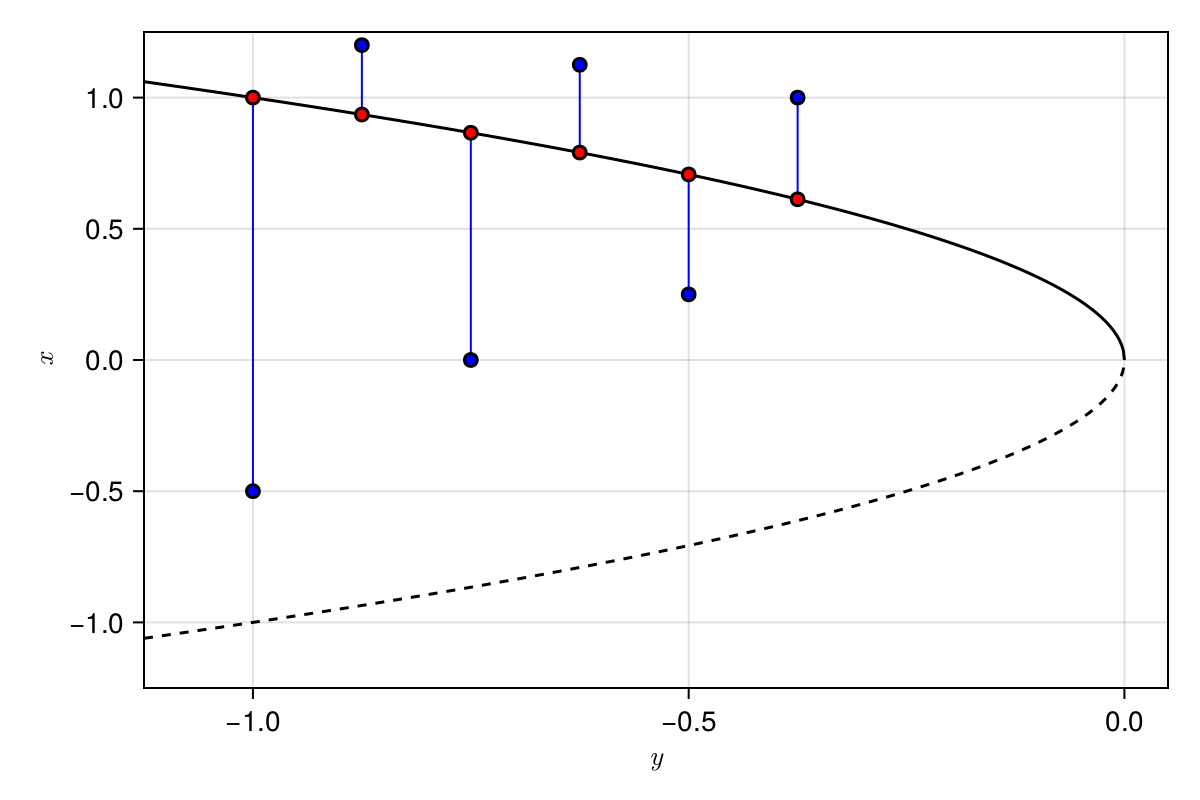
\includegraphics[keepaspectratio, width=0.75\textwidth]{../figures/FoldFast.png}
        \caption{Trajectories of the fast subsystem in phase space for different initial conditions (blue dots) each attracted to the corresponding equilibria (red dots) on the stable submanifold (solid black line).}
        \label{fig1.1}
    \end{figure}
   \begin{figure}[H]
        \centering 
        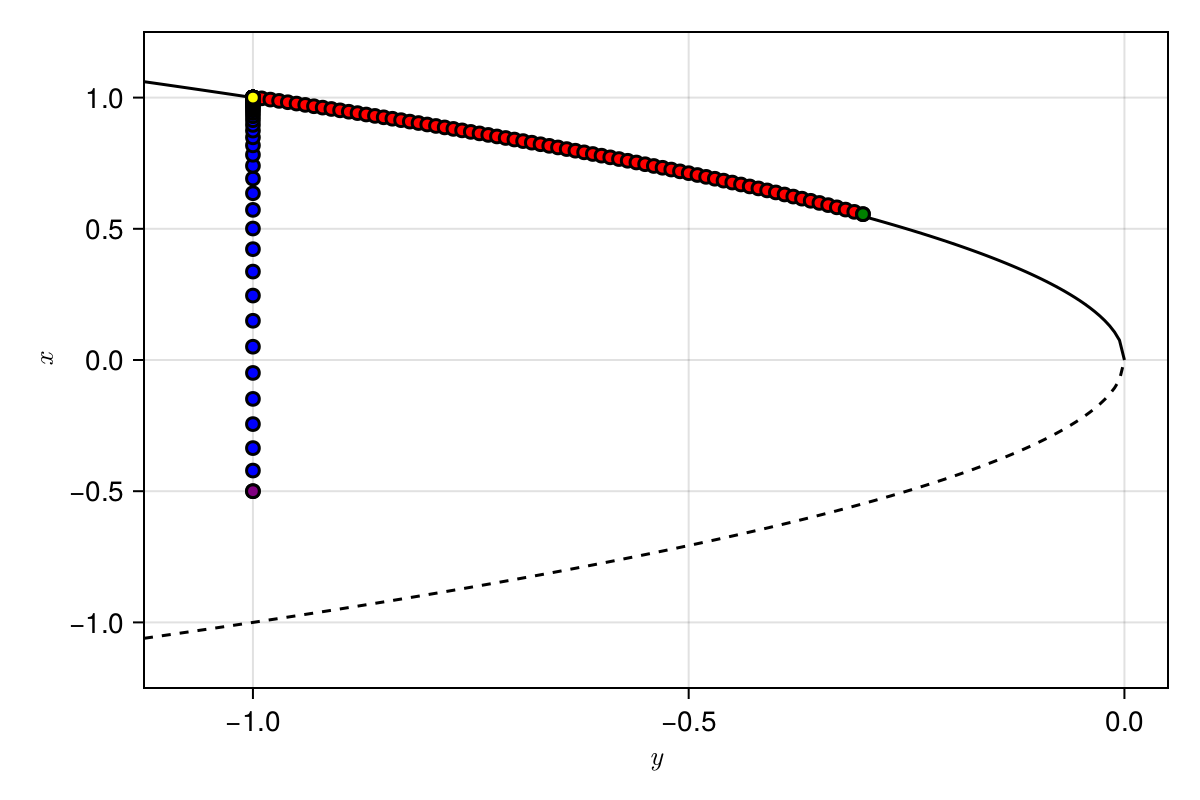
\includegraphics[keepaspectratio, width=0.75\textwidth]{../figures/Fold.png}
        \caption{Trajectory of the layer equation (blue dots) starting at initial condition $(x=-0.5,y=-1)$ (purple dot) and ending on the attracting submanifold (yellow dot). The resulting final state $(x=1,y=-1)$ is then chosen as the initial condition for the evolution of the reduced equation whose trajectory (red dots) stay on the critical manifold for until reaching the final state (green dot).}
        \label{fig1.2}
    \end{figure}
 \end{example_continued}
 \begin{example_continued}{}{}
   \begin{figure}[H]
       \centering 
       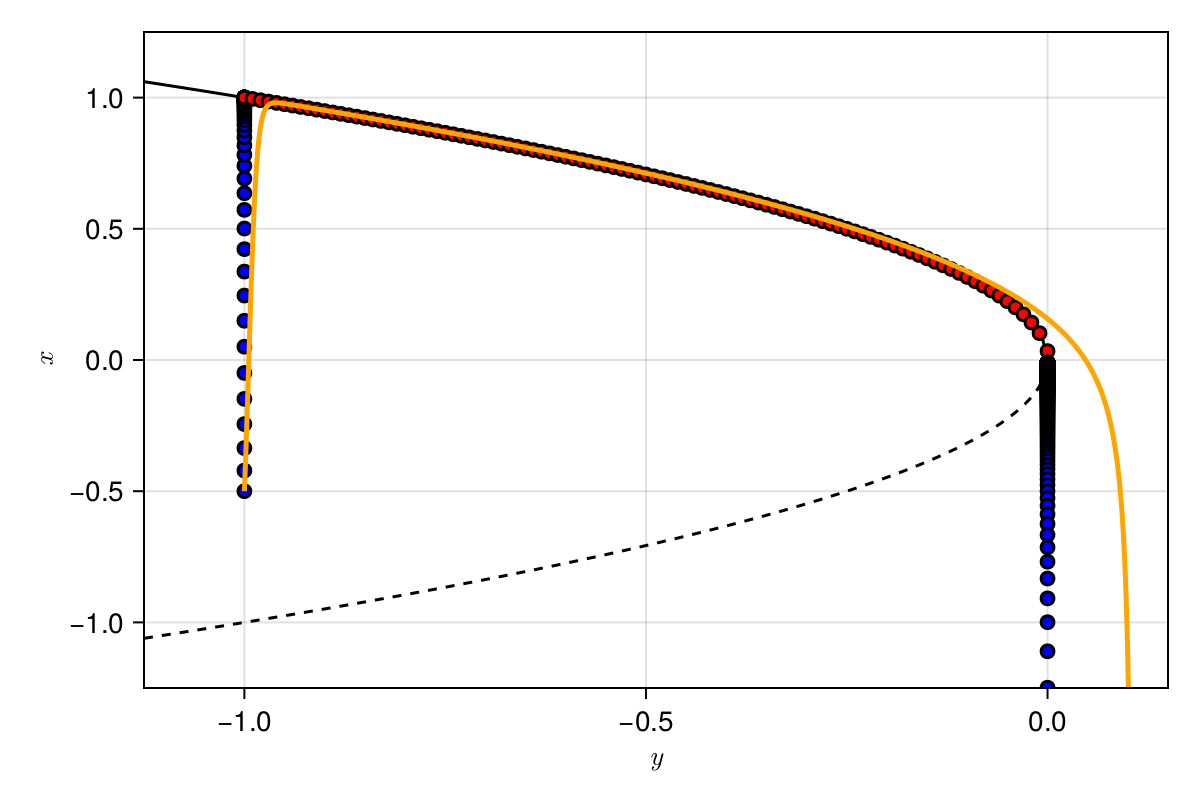
\includegraphics[keepaspectratio, width=\textwidth]{../figures/FoldFastSlow.png}
       \caption{Comparison between a concatenation of fast (blue dots) and slow (red dots) subtrajectories in the singular limit with a fast-slow trajectory in the non-singular regime (yellow solid line) computed with a timescale value of $\epsilon=1\cdot10^{-2}$. Note how the subtrajectories in the singular limit constitute an ideal approximation of the real (numerically computed) fast-slow trajectory with the latter featuring a delay in the critical transition (fold bifurcation at $x=0$) which can be quantified using Theorem \ref{thm1.2} and \ref{thm1.2}.}
       \label{fig1.3}
   \end{figure}
 \end{example_continued}
Sometimes, depending on the fast dynamics, it is even possible to reconstruct the fast flow $x(\tau)$ from the reduced equation thanks to a set of important results in geometric singular perturbation theory \cite{Wechselberger20}.
\begin{theorem}[label=thm1.1]{Implicit Function Theorem}{}
     Let \eqref{eq1.1} be a fast-slow system and \eqref{eq1.5} its critical manifold, then if $C$ is normally hyperbolic (i.e. the Jacobian $D_{x}f$ is hyperbolic and all its eigenvalues have non-zero real parts) then there exists a map $h:y\mapsto x$ s.t. $f(h(y),y)=0$.
\end{theorem}
\begin{theorem}[label=thm1.2]{Fenichel's $(1^{st})$ Theorem}{}
     Let $C$ be a compact, normally hyperbolic manifold then for $\epsilon>0$ sufficiently small there exists $C_{\epsilon}$ locally invariant and diffeomorphic to $C$ that lies at a Hausdorff distance $O(\epsilon)$ from $C$.
\end{theorem}
Those results allow us to fully characherize the critical manifold in terms of both the fast and slow variables
\begin{equation}\label{eq1.6}
        C=\{(x,y)\in \mathbb{R}^{n+m}\;:\;h(y)=x\,,\;f(h(y),y)=0\}\,,
\end{equation}
while also at the same time providing us with a convenient way to construct (infinitely many) singulalry perturbed manifolds 
\begin{equation}\label{eq1.6.2}
        C_{\epsilon}=\{(x,y)\in \mathbb{R}^{n+m}\;:\;x=h_{\epsilon}(y)=h(y)+O(\epsilon)\}\,
\end{equation}
to which the critical manifold $C$ deforms to in the singular limit $\epsilon\to0$.
Finally we observe that, as briefly mentioned in Example $(\ref{ex1.1})$, in the singular limit we can derive an approximation of the fast-slow dynamics by chaining together fast and slow trajectories, the latter being constrained onto the critical manifold while the former being a trivial evolution of the layer equation for fixed values of the parameter $y$.
These links between fast and slow trajectories do in fact provide us an initial albeit intuitive definition of transitions in the fast-slow dynamical system in which we can observe an abrupt switch between fast and slow evolution and viceversa.  
By remarking that any trajectory onto the critical manifold is, by definition, a slow flow solving the reduced equation, we can then easily deduce that a transition between a slow to fast (repelling) dynamics is necessarily a critical transition for the dynamical system. As such any concatenation of a slow flow final state with a fast flow initial condition uniquely identifies a critical transition.
\begin{definition}[\hl{Critical transition}]\label{def1.3}
        Let $\gamma(t)$ be a homeomorphic image of the real subset $(a,b)$ s.t. for each partitioning ${a=t_{0}<t_1,\dots,t_{N-1}<t_N=b}$ the image $\gamma(t_{j-1},t_j)$ is an orientation preserving trajectory of either the layer \eqref{eq1.3} or the reduced equation \eqref{eq1.4} and let $p\in C$ be a point where the critical manifold loses its normal hyperbolicity, then $p$ is a critical transition if there exist a candidate trajectory $\gamma$ s.t. $p = \gamma(t_j)$ is a transition between fast and slow regimes and $\gamma(t_{j-1},t_j)$ is normally hyperbolic and attracting.
\end{definition}
\subsection{Embedding stochasticity in the system}\label{subsec2.2}
Motivated by many physical applications, in which the underlying dynamical system appears to be perturbed by noise, we will now consider stochastic differential equations (SDEs) as our starting point in dealing with temporal critical transitions.
\begin{definition}[\hl{Stochastic fast-slow system}]\label{def1.4}
     Let $V:=(\Omega,\mathcal{F},\mathbb{P})$ be a probability space and $W=(W_1, \dots, W_n)$ a $n-$dimensional Brownian motion with components in $V$ then
     \begin{equation}\label{eq1.7}
        \begin{cases}
           dx = \epsilon^{-1} f(x,y)d\tau + \sigma_f(x,y)dW \,, \\
           dy = g(x,y)d\tau + \sigma_g(x,y)dW \,, 
        \end{cases}
     \end{equation}
     is a stochastic fast-slow system in the slow timescale $\tau:=\epsilon t$ with deterministic dynamics $f,g$ and stochastic dynamics $\sigma_f,\sigma_g$. 
\end{definition}
The system in \eqref{eq1.7} is said to be in Itô differential form; if both the fast $\sigma_f(x,y)=\sigma_f\in\mathbb{R}$ and slow $\sigma_g(x,y)=\sigma_g\in \mathbb{R}$ stochastic dynamics are constants then we are dealing with an Ito's SDE with additive noise, otherwise it will be characterised by multiplicative noise.
Let us first consider the former case for which the stochastic fast-slow system reads
\begin{equation}\label{eq1.8}
   \begin{cases}
      dx = \epsilon^{-1} f(x,y)d\tau + \frac{\sigma_f}{\sqrt{\epsilon}}\,dW\,, \\
      dy = g(x,y)d\tau + \sigma_g\,dW \,, 
   \end{cases}
\end{equation}
where we notice the scaling of the noise for the fast equation due to the scaling law of Brownian motion i.e. $W(\tau)=W(\epsilon t)=\sqrt{\epsilon}W(t)$.
For \eqref{eq1.8} we would like to use the results derived in the previous subsection for the deterministic case and in particular our aim is to characterise the time evolution in terms of concatenations of separated fast and slow trajectories.
To that end let us use Definition \ref{def1.3} and analyse the stochastic fast-slow system in order to identify the regions of $y$ close to a critical transition from those that are far away. 
Accordining to the definition, a sample path realised from \eqref{eq1.8} is away from a critical transition as long as it stays close (in probabilistic terms) to the portion of the critical manifold $C$ that is normally hyperbolic and attracting, i.e. $C^{(a)}$.
From Theorem \ref{thm1.2} we can uniquely identify the slow manifold $C_{\epsilon}$, as reported in \eqref{eq1.6.2}, by constructing the map $h_{\epsilon}(y)=h(y) + O(\epsilon)$; it is thus intuitive to define a new stochastic process $\xi(\tau)=x(\tau)-h_{\epsilon}(y)$ which quantifies the concentrations of realizations of the sample path from \eqref{eq1.8} that stay close to $C^{(a)}$. We then apply Ito's formula to this new process to derive the associated SDE; after that we define once again a new stochastic process $X(\tau):=\sigma_f^{-2} \text{Var}(\xi)$ which satisfies the following deterministic fast-slow system
\begin{equation}\label{eq1.9}
   \begin{cases}
      \dot{X} = 2\epsilon^{-1}A_{\epsilon}(y)X +1 \,, \\
      \dot{y} = g(h_{\epsilon}(y),y) \,, 
   \end{cases}
\end{equation}
with $A_{\epsilon}(y)=(D_x f)(h_{\epsilon}(y),y) - \epsilon (D_y h_{\epsilon})(y) (D_x g)(h_{\epsilon}(y),y)$. Applying Theorem \ref{thm1.2} again for \eqref{eq1.9} we can construct a new slow manifold for the sample paths of the new stochastic fast-slow system
\begin{equation}\label{eq1.10}
        C_{\epsilon}^{(X)}:=\{(X,y)\in \mathbb{R}^2\;:\;X=H_{\epsilon}(y):=- \frac{1}{2A_{\epsilon}(y)+O(\epsilon)}\}\,,
\end{equation}
and from that we finally can define a neighborhood of the slow manifold which scales with the variance of sample paths
\begin{equation}\label{eq1.11}
        N(\rho;C_{\epsilon}):=\{(x,y)\in \mathbb{R}^{2}\;:\;\frac{(x-h_{\epsilon}(y))^{2}}{H_{\epsilon}(y)}<\rho^2\}\,.
\end{equation}
This object provides us with a convenient criterion to discriminate the sample paths of the stochastic fast-slow system that are away from the critical transitions, for which the sample paths stay bounded within $N(\rho;C_{\epsilon})$.
\begin{theorem}[label=thm1.3]{}{}
    Let \eqref{eq1.8} be a stochastic fast-slow system with additive noise then its sample paths whose initial conditions are on the slow manifold $C_{\epsilon}$ stay bounded within the neighborhood $N(\rho;C_{\epsilon})$ with high probability. 
\end{theorem}
We are now able to charactere noise-induced critical transitions (N-tipping) with an equivalent relation to the deterministic case (i.e. B-tipping) derived in the previous section.
\begin{interpretation*}{}
     According to Definition \ref{def1.3} the slow subtrajectory of the sample paths will stay bounded within $N(\rho;C_{\epsilon})$ as it will pass through a region of $y$ close to a normally hyperbolic and attracting submanifold $C^{(a)}$ while approaching a critical transition when the regime shifts from slow attracting to fast repelling. Since $N(\rho;C_{\epsilon})$ scales with the variance we are expecing the sample paths to escape such region, as they approach a critical transition, with higher probabilities, meaning that the variance should increase the closer the paths get to the tipping point. This increase in variance can thus be interpreted as an EWS for B- and N-tipping affecting stochastic fast-slow systems with additive noise.
\end{interpretation*}
Finally we notice that a trivial rescaling and coordinate transformation will allow us to recast any sample path away from the critical transitions in the following stochastic fast-slow system
\begin{equation}\label{eq1.12}
   \begin{cases}
      dx = -\epsilon^{-1}\alpha x d\tau + \frac{\sigma}{\sqrt{\epsilon}}dW \,, \\
      dy = d\tau \,, 
   \end{cases}
\end{equation}
which is the Ornstein-Uhlenbeck process (OUP) with linear drift $(0<\alpha=0(1))$ and constant diffusion $(\sigma_f=:\sigma>0)$.
With these results we are now capable to fully distinguish states of the sample paths of stochastic fast-slow systems that are on normally hyperbolic and attracting submanifolds as stable regimes that are far away from the critical transitions. It will become fundamental later, when deriving stochastic indicators for such transitions, how we choose an appropriate criterion that will count a sample path as escaped fron the slow manifold $C_{\epsilon}$ and therefore linking together such indicators with the OUP normal form derived in this section. 
\begin{example}[label=ex1.2]{}{}
        Let us consider a sample path realised by the OUP in \eqref{eq1.12} with drift constant $\alpha=1$, timescale constant $\epsilon=2\cdot10^{-2}$ and noise level $\sigma=0.1$. 
        We want to construct the neighborhood $N(\rho;C_{\epsilon})$ in \eqref{eq1.11} for such case and confirm that the numerical sample paths stay in fact bounded within such neighborhood with high probability. 
        To do so we must first construct the (deterministic) slow manifold $C_{\epsilon}$ and for that we need in turn to derive the map $h_{\epsilon}(y)=h(y)+O(\epsilon)$ which uniquely identifies it as per Fenichel's first Theorem \ref{thm1.2}. 
        With the critical manifold coinciding with the $y-$axis
        \begin{equation*}
            C=\{(x,y)\in \mathbb{R}^{2}\;:\;f(x,y)=-\alpha x = 0\:\Rightarrow\: x=0\;\forall \alpha\neq0,\,\forall y\in \mathbb{R}\}\,,
        \end{equation*}
        we can easily check that the existance of $h:y\mapsto x$ is guranteed by Theorem \ref{thm1.1} given that $C$ is normally hyperbolic at any point.
        It follows similarly that the only map $x=h(y)=0,\:\forall y\in \mathbb{R}$ is the null function yielding 
        \begin{equation*}
                h_{\epsilon}(y) = h(y) + O(\epsilon) = O(\epsilon)\quad\Longrightarrow\quad C_{\epsilon}=\{(x,y)\in \mathbb{R}^{2}\;:\;x=O(\epsilon)\}\,.
        \end{equation*}
        This tells us that the slow manifold is a narrow strip wrapped around the critical manifold whose width is twice the Hausdorff distance from $C$.
        The next step in our construction is to derive a new slow manifold $C_{\epsilon}^{(X)}$ for the process 
        \begin{equation*}
             X=\sigma^{-2}\text{Var}(\xi)=\sigma^{-2}\text{Var}(x - h_{\epsilon}(y))=\sigma^{-2}\text{Var}(x)\,,
        \end{equation*}
        where we recall the invariance of the variance under additive constant perturbations.
        First we compute the quantity $A_{\epsilon}(y)=(D_x f)(h_{\epsilon}(y),y) - \epsilon (D_y h_{\epsilon})(y) (D_x g)(h_{\epsilon}(y),y)=-\alpha$ and then by using \eqref{eq1.10} we get
        \begin{equation*}
                C_{\epsilon}^{(X)}=\{(X,y)\in \mathbb{R}^{2}\;:\;X=\frac{1}{2 \alpha}+O_{1}\epsilon\}\,.
        \end{equation*}
        Now, according to \eqref{eq1.11}, we can finally construct the neighborhood
        \begin{equation}\label{eq1.13}
                N(\rho;C_{\epsilon})=\{\frac{\sigma^{-2}\text{Var}(x)+O_{2}(\epsilon)}{\frac{1}{2 \alpha}+O_{1}(\epsilon)}<\rho^{2}\}=\{\frac{\sigma^{-2}\text{Var}(x)+M_{2}\epsilon}{\frac{1}{2 \alpha}+M_{1}\epsilon}<\rho^{2}\}\,,
        \end{equation}
        for which $M_{1}, M_{2}$ are two distinct, positive constants that need to be quantified in order to compute $\rho$ which will give us the boundaries $\partial N(\rho;C_{\epsilon})=\sqrt{\rho^{2}}$.
        To do so let's observe that $X=H_{\epsilon}(y)=\frac{1}{2A_{\epsilon}(y)}+O_{1}(\epsilon)\;\Rightarrow\;|X|=|\sigma^{-2}\text{Var}(x)|< M_{1}\epsilon$.
        We recall that $x(\tau)$ is in fact an OUP for which we have an analytical expression for its variance readily available
        \begin{equation}\label{eq1.14}
             \text{Var}(x(\tau)) = (x_0 - \frac{\sigma^2}{2 \alpha})e^{-2\frac{\alpha\tau}{\epsilon}}\,.
        \end{equation}
        We can the plug in the values for $\alpha,\,\sigma$ and $\epsilon$ in \eqref{eq1.14} to get $M_{1}=225$.
        Similarly for the other constant we get $x=h_{\epsilon}(y)=O_{2}\;\Rightarrow\;|x|<M_{2}\epsilon$; here we assume that $\underset{\tau\in \mathbb{R}^{+}}{\text{max}}|x(\tau)|=0.25$ which lead us to the value $M_{2}=12.5$. Putting al together into \eqref{eq1.13} finally gives us $\rho = \pm 0.35$.
\end{example}
\begin{example_continued}{}{}
        We are now able to compute the closure of the neighborhood $N(\rho;C_{\epsilon})$ of the critical manifold $C_{\epsilon}$ within which our sample paths $x(\tau)$ for the OUP (which are normally distributed) will stay bounded with high probability.
     \begin{figure}[H]
         \centering 
         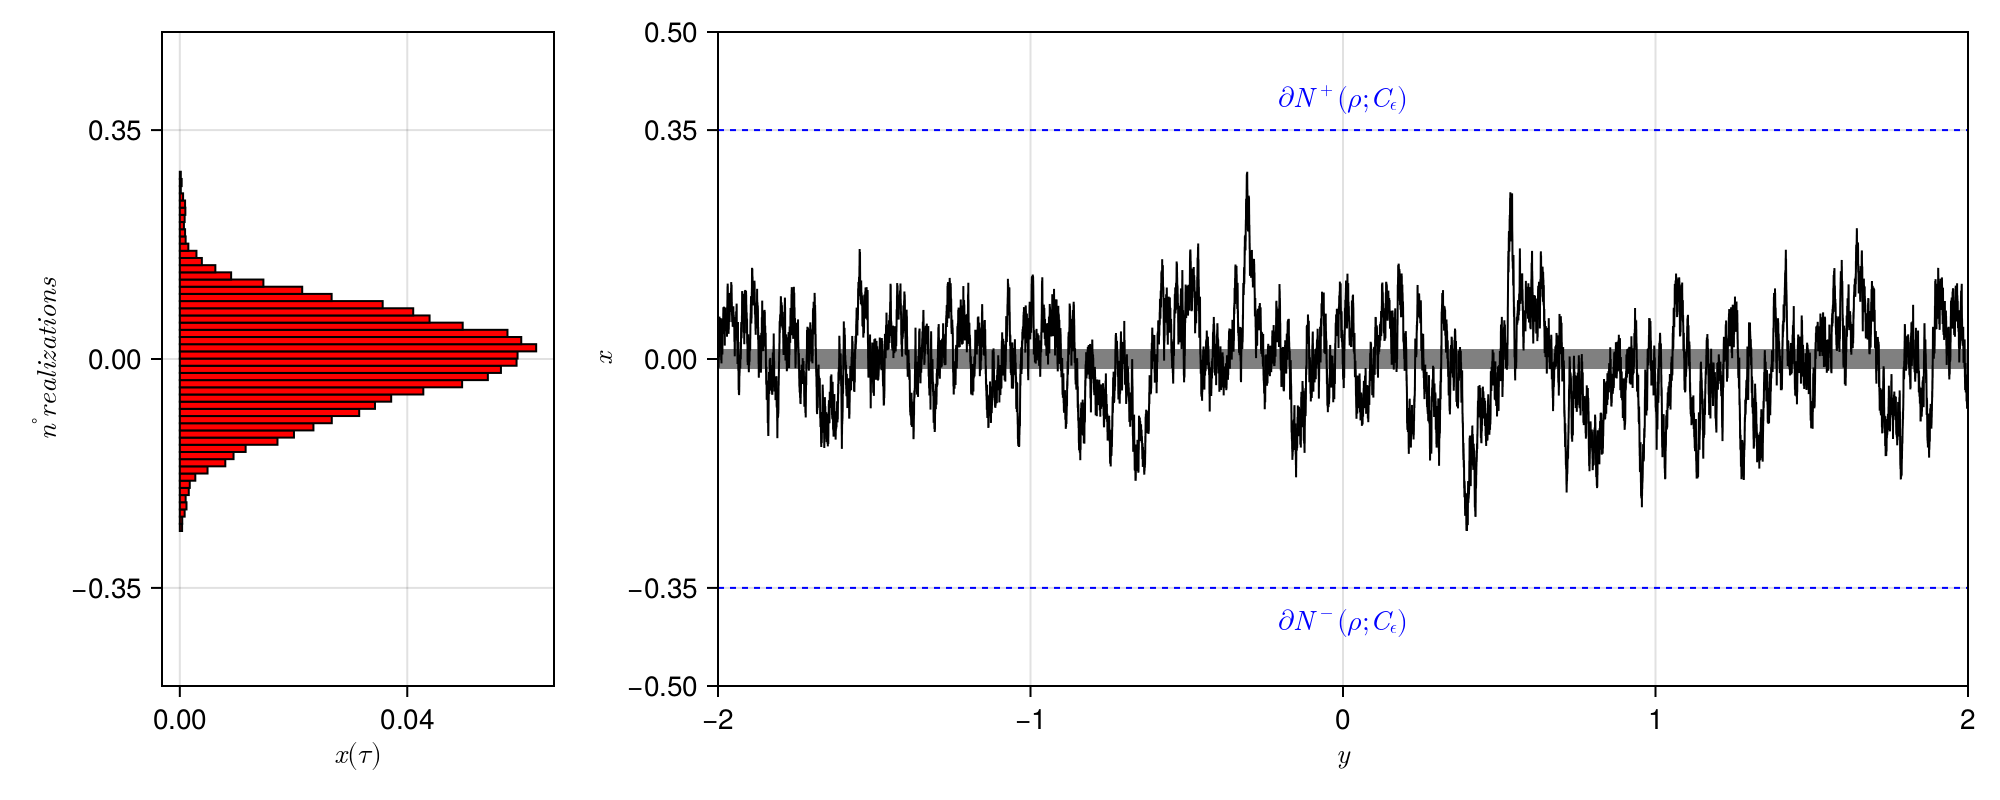
\includegraphics[keepaspectratio, width=\textwidth]{../figures/OUP.png}
         \caption{Sample path of the OUP starting on the slow manifold $C_{\epsilon}$ (gray strip). Note how the fast variable stays bounded within the neighborhood $N(\rho;C_{\epsilon})$ (dashed blue lines) with probability $1$ for all of the (fixed) values of the slow variable $y$.}
         \label{fig1.4}
     \end{figure}
     \begin{figure}[H]
         \centering 
         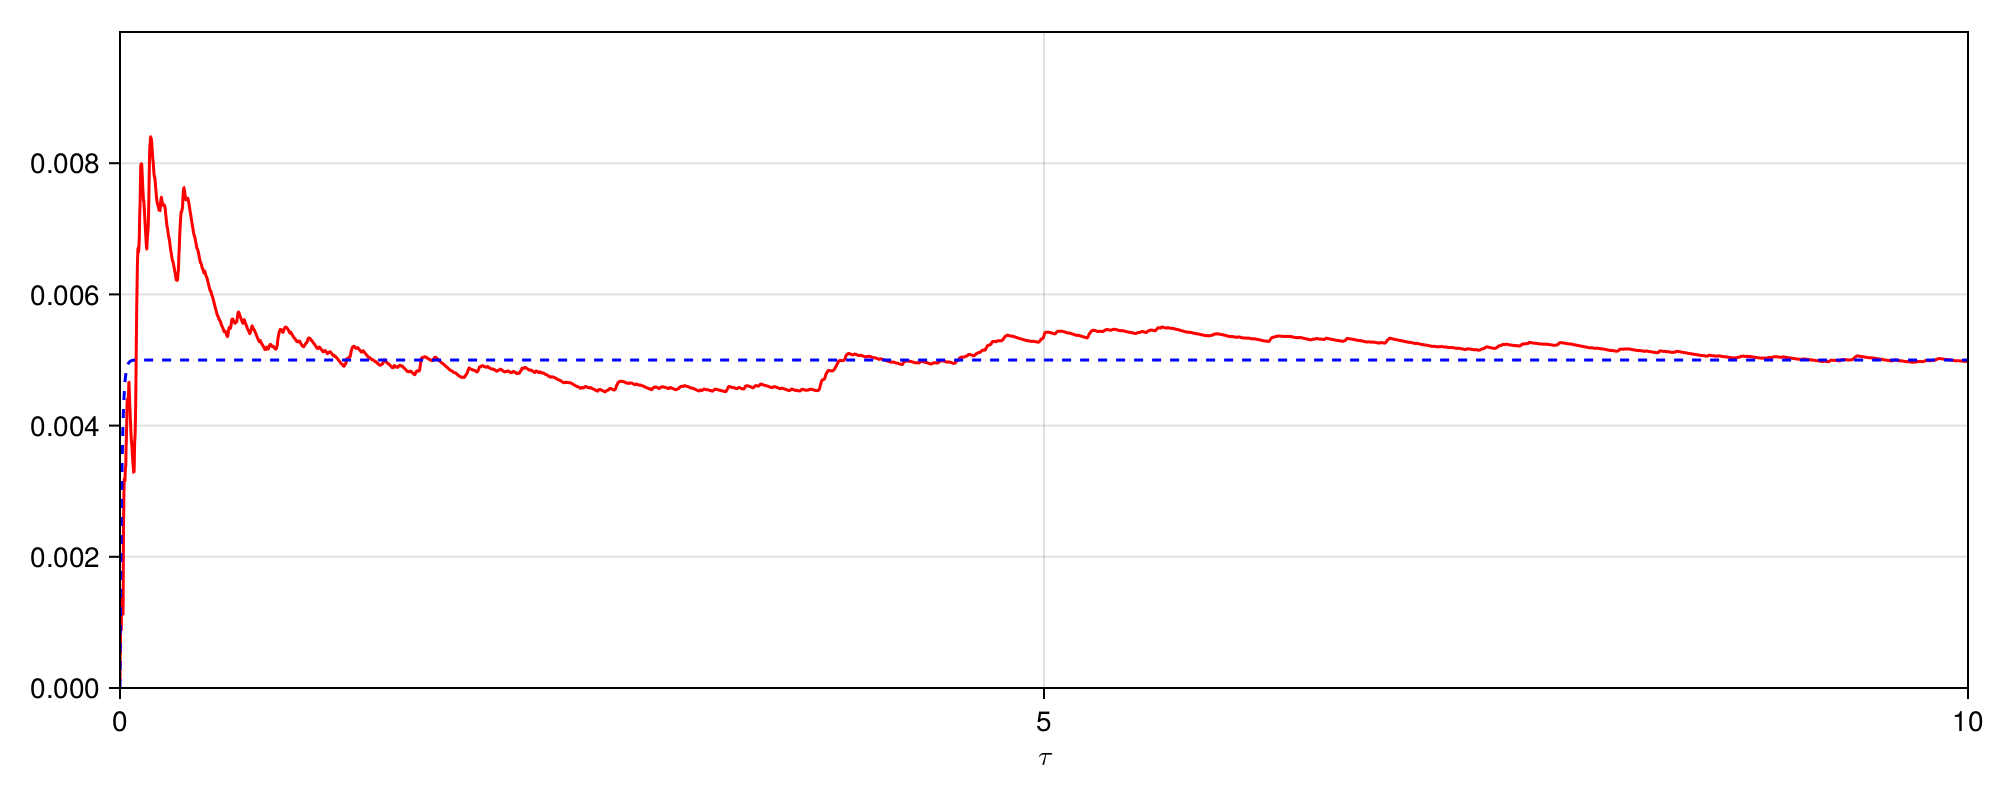
\includegraphics[keepaspectratio, width=\textwidth]{../figures/OUP-var.png}
         \caption{Comparison of the analytical variance (dashed blue line) of the OUP process derived in \eqref{eq1.14} with the numerical variance (solid red line) computed from the sample path showing asymptotic convergence.}
         \label{fig1.5}
     \end{figure}
\end{example_continued}
\subsection{Predicting noise-induced critical transitions}\label{subsec2.3}
We are now concerned in characterising the sample paths for those stochastic fast-slow systems that are instead close to or approaching the tipping point. Theorem \ref{thm1.3} already gives us a first hint by identifying the increase in variance of the time-series as the neighborhood $N(\rho;C_{\epsilon})$ grows in size while approaching the B-tipping. 
To deal with this problem in more general terms let us abandon the sample path point of view and consider instead possibile qualitative changes in the Fokker-planck distribution associated to an ensemble of stochastic processes of the form \eqref{eq1.7}.
\begin{definition}[\hl{Phenomenological bifurcation}]\label{def1.5}
     Let \eqref{eq1.7} be a stochastic fast-slow system and $p_{s}(x,y)$ be a probability density for the stochastic process defined by \eqref{eq1.7} satysfing the stationary Fokker-Plank equation \eqref{eq0.1} then $y=y_{p}$ is a phenomenological bifurcation if $p_{s}(x,y<y_{p})$ is qualitatively different from $p_{s}(x,y>y_{p})$. 
\end{definition}
\begin{example}[label=ex1.3]{}{}
     We consider the case for a stochastic fast-slow system in the fast timescale, i.e.
     \begin{equation*}
        \begin{cases}
            dx = f(x,y)\,dt + \sigma_{f}(x,y)\,dW\,, \\
            dy = \epsilon g(x,y)\,dt + \sigma_{g}(x,y)\,dW\,. 
        \end{cases}
     \end{equation*}
     Taking the singular limit, we reduce the above to the (stochastic) layer equation
     \begin{equation*}
         dx =  f(x,y)\,dt + \sigma_{f}(x,y)\,dW\,,
     \end{equation*}
     for fixed values of the parameter $y\in \mathbb{R}$. We now specify a multiplicative noise stochastic dynamics for the transcritical normal form, i.e.
     \begin{equation}\label{eq1.15}
         dx = (yx - x^{2} + \frac{1}{2}\sigma^{2}x)\,dt + \sigma x\,dW\,. 
     \end{equation}
     This case was first introduced in \cite{Arnold98} in the context of studying potential bifurcations by tracking the convergence of invariant measures for parametrised families of random dynamical systems. 
     What we will do instead is verify whether a qualitative change in the stationary Fokker-Planck distribution of this process occurs as the transcritical bifurcation point $y=0$ is approached. From \eqref{eq0.1} we write the stationary Fokker-Planck equation associated to \eqref{eq1.15}
     \begin{equation}\label{eq1.16}
          0 = -\frac{d}{dx}((yx - x^{2} + \frac{1}{2}\sigma x)p_{s}(x; y)) + \frac{d^{2}}{dx^{2}}(\frac{1}{2}\sigma^{2}x^{2}\,p_{s}(x; y))\,,
     \end{equation}
     whose solution, for $x>0$ is the Gamma distribution
     \begin{equation}\label{eq1.17}
          p_{s}(x; y) = \frac{1}{N_{y}}\,x^{\frac{2y}{\sigma^{2}}-1}\,e^{-\frac{2x}{\sigma^{2}}}\,,\quad N_{y}=\int_{0}^{+\infty} x^{\frac{2y}{\sigma^{2}}-1}\,e^{-\frac{2x}{\sigma^{2}}}\,dx = (\frac{\sigma^{2}}{2})^{\frac{2y}{\sigma^{2}}}\,\Gamma(\frac{2y}{\sigma^{2}})\,. 
     \end{equation}
     We can easily conclude that \eqref{eq1.17} is unimodal in the parameter range $y\in(0, \frac{\sigma^{2}}{2})$ and it undergoes a clear qualitative change for parameter values $y>\frac{\sigma^{2}}{2}$. The parameter value $y_{p}=\frac{\sigma^{2}}{2}$ is therefore a phenomenological bifurcation for our transcritical normal form. 
     Both mean and variance of the Gamma distribution are linear in $y$ and specifically
     \begin{equation*}
         \mathbb{E}(x; y)=y\,,\quad \text{Var}(x; y) = \frac{\sigma^{2}}{2}\,y\,,
     \end{equation*}
     which is in agreement with the fact that sample paths that stay bounded after the transcritical bifurcation in $y=0$ will follow the stable branch of the manifold. 
\end{example}
\begin{example_continued}{}{}
     \begin{figure}[H]
         \centering 
         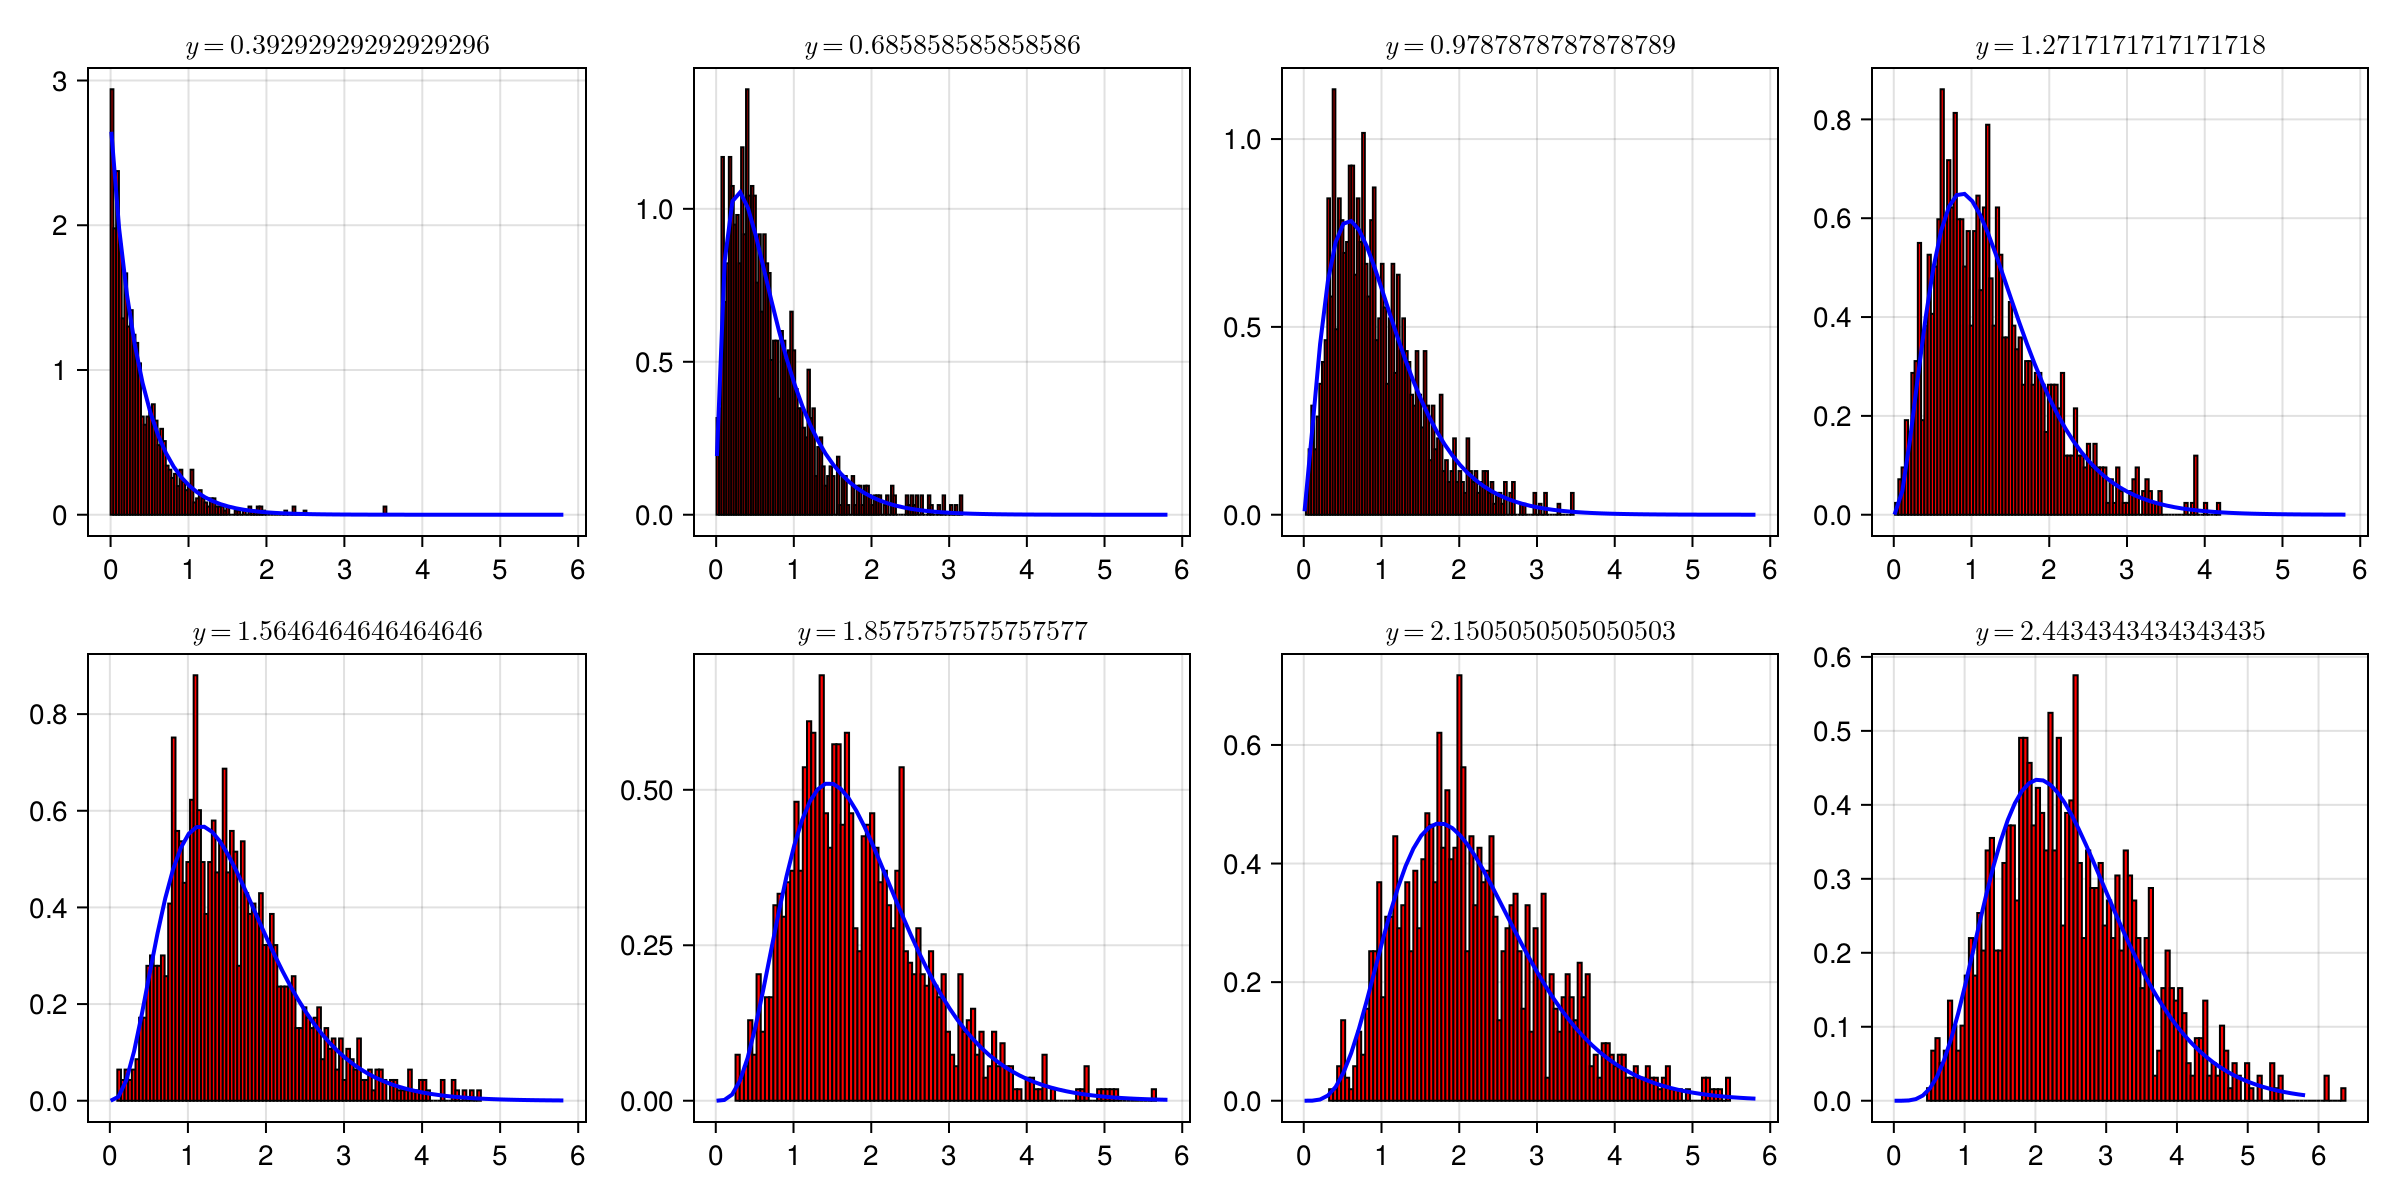
\includegraphics[keepaspectratio, width=\textwidth]{../figures/MultDistro.png}
         \caption{Plots of the stationary Fokker-Plank distribution \eqref{eq1.17} (solid blue lines) for a transcritical normal form with (multiplicative) noise level $\sigma = \sqrt{0.8}$ for different values of the parameter overlayed with histograms (red bars) associated to an ensemble simulation of $1000$ sample paths \eqref{eq1.15}. 
         Notice how from the top left, corresponding to a parameter value of $y<y_{p}=0.4$, to every other snapshot in the picture, the density undergoes a qualitative change from singular (unimodal) to non-singular.}
         \label{fig1.6}
     \end{figure}
     \begin{figure}[H]
         \centering 
         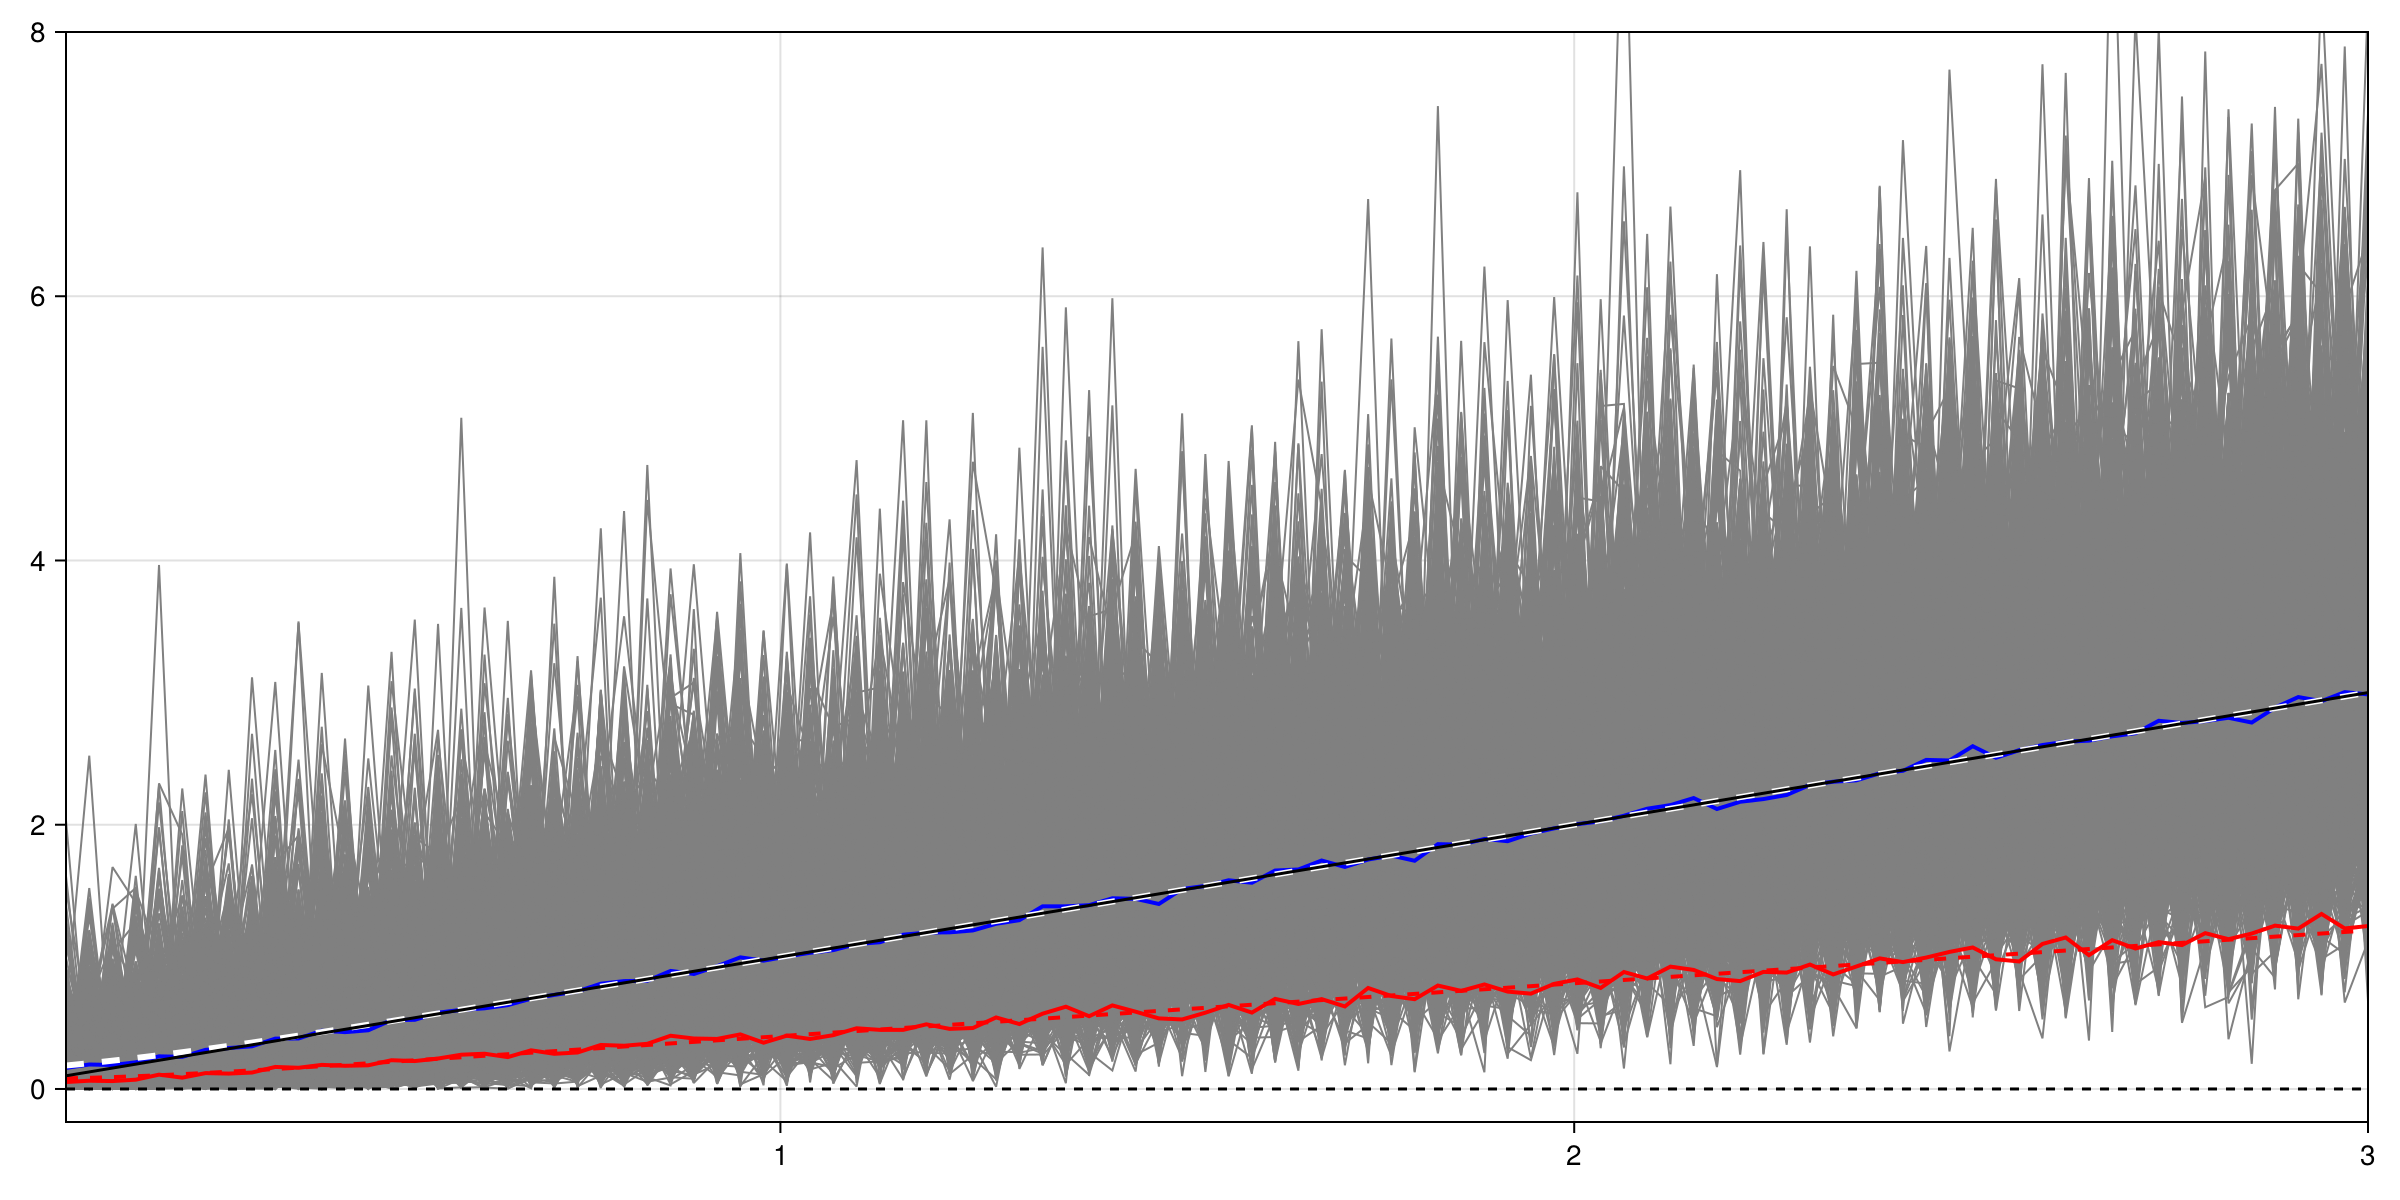
\includegraphics[keepaspectratio, width=0.95\textwidth]{../figures/MultEnsemble.png}
         \caption{Plot of the $1000$ sample paths (grey lines) of the ensemble simulation of \eqref{eq1.15} in the augmented state space superimposed to their mean (white dashed line for the analytical value and solid blue line for the numerical one) and variance (dashed red line for the analytical value and solid red line for the numerical one).
         Notice how the (analytical) mean follows exactly the stable branch of the critical manifold following the transcritical bifurcation.}
         \label{fig1.7}
     \end{figure}
\end{example_continued}
We are now equipped with a criterion to discern those sample paths that are away from the critical transition from those approaching it; in both cases we observed that the variance of the ensemble constitutes an EWS to predict the upcoming B-tipping. 
Since we established earlier that sample paths away from the transitions can be modelled as the OUP we can therefore still safely rely on the approach of monitoring the Fokker-Planck distribution for paths that are instead close to the tipping point. 
To do that in the most general approach we need to specify appropriate boundary conditions for the Fokker-Planck equation in order to properly capture and separate sample paths that have escaped the attracting submanifold from those that instead stay bounded to it.
As such, considering a layer equation of the form \eqref{eq1.3} we write the associated Fokker-Planck equations
\begin{equation}\label{eq1.18}
     \partial_{t}p(x,t) = -\partial_{x}J(x,t) \,,
\end{equation}
where $J(x,t):= f(x,y)p(x,t) - \frac{\sigma^{2}}{2}\partial_{x}p(x,t)$ is the probablity density current. The fundamental assumption here is that there exist a stationary (asymptotic) state for the stochastic process (for simplicity we consider the case of additive noise) 
\begin{equation*}
    dx = f(x,y)\,dt + \sigma\,dW\,,
\end{equation*}
whose distribution satisfies the stationary limit of \eqref{eq1.18}
\begin{equation}\label{eq1.19}
     \newprime{J}(x) = 0\;\Rightarrow\; J(x) = \text{constant}(x)\,. 
\end{equation}
We immediately realise that equation \eqref{eq1.19} is defined over the entirety of the real (spatial) domain, meaning that in order to restrict it to a bounded and limited subinterval $[a,b]\subset \mathbb{R}$ we must enforce the entirety of the probability current to never leave such domain, resulting in the specification of reflecting boundary conditions. 
The reason for this immediately follow by the constraint of the stationary Fokker-Planck density to remain normalised in any subdomain $[a,b]$ we restrict ourselves to.
Following the imposition of reflecting boundary conditions we get that the only possible constant that satisfies \eqref{eq1.19} is $J(x)=J=0$. From the definition of $J(x,t)$ this leads to a first-order, homogeneous, non-linear ODE whose general integral can be explicitly calculated
\begin{equation}\label{eq1.20}
     p(x)=\frac{1}{N}\,e^{2 \int_{a}^{x}\frac{1}{\sigma^{2}}f(u,y)du}\,,\quad N = \int_{a}^{b}\int_{a}^{v}\frac{1}{\sigma^{2}}f(u,y)du\,dv\,.
\end{equation}
The above stationary Fokker-Planck distribution gives us a convenient method to detect potential phenomenological bifurcation by tracking the parameter evolution of the distribution; this result has an important practical value since we don't necessarly need to know the deterministic dynamic $f(x,y)$ to observe a qualitative change in \eqref{eq1.20} as long as our ensemble simulations are reliable.
Nevertheless, since visually monitoring the distribution histogram is not always a practical nor sometimes available solutions in real-life applications more quantitative measures need to be derived from \eqref{eq1.20} as a more robust EWS.
As already mentioned above, the variance has insofar provided a good signal to anticipate and predict the critical transition. From \eqref{eq1.20} we specify any normal form $f(x,y)$ and check wether the associated variance is indeed a good EWS for the associated deterministic bifurcation.
Here we will only consider the following three cases
\begin{table}[H]
\centering
\begin{tabular}{|c|c|c|c|}
 \hline
 Normal form & $f(x,y)$ & $p_{s}(x;y)$ & Boundaries \\
 \hline
 Fold & $-y - x^{2}$ & $\frac{1}{N_{\text{fold}}}\,e^{\frac{2}{\sigma^{2}}(-yx - \frac{1}{3}x^{3}+\frac{2}{3}(-y)^{\frac{3}{2}})}$ & $a = -\sqrt{-y}$, $b = \infty$ \\
 Pitchfork & $yx - x^{2}$ & $\frac{1}{N_{\text{pitch}}}\,e^{\frac{2}{\sigma^{2}}(\frac{1}{2}yx^{2} - \frac{1}{3}x^{3}-\frac{1}{6}y^{3})}$ & $a = y$, $b = \infty$ \\
 Transcritical & $yx + x^{3}$ & $\frac{1}{N_{\text{trans}}}\,e^{\frac{2}{\sigma^{2}}(\frac{1}{2}yx^{2} + \frac{1}{4}x^{4}+\frac{1}{4}y^{2})}$ & $a = -\sqrt{-y}$, $b = \sqrt{-y}$ \\
 \hline
 \end{tabular}
 \end{table}
 We highlight how the specified choices for each boundary is made in order to enforce reflecting boundary conditions for the Fokker-Planck stationary density. In practice however, when we're dealing with ensemble simulations, we will specify the unstable branch of each critical manifold as the boundary for the sample paths of each normal form and a trajectory that crosses beyond such boundary is counted as escaped (N-tipping).
In Figure \ref{fig1.8} we plot the analytical variance computed from each distribution against the numerical variance computed from an ensemble of $1000$ sample paths. It is clear how the choice of reflecting boundary conditions is necessary for the computation of the variance in the context of deriving an EWS for a deterministic critical transition (B-tipping).
\begin{figure}[H]
    \centering 
    \begin{subfigure}[b]{0.3\textwidth}
        \centering 
        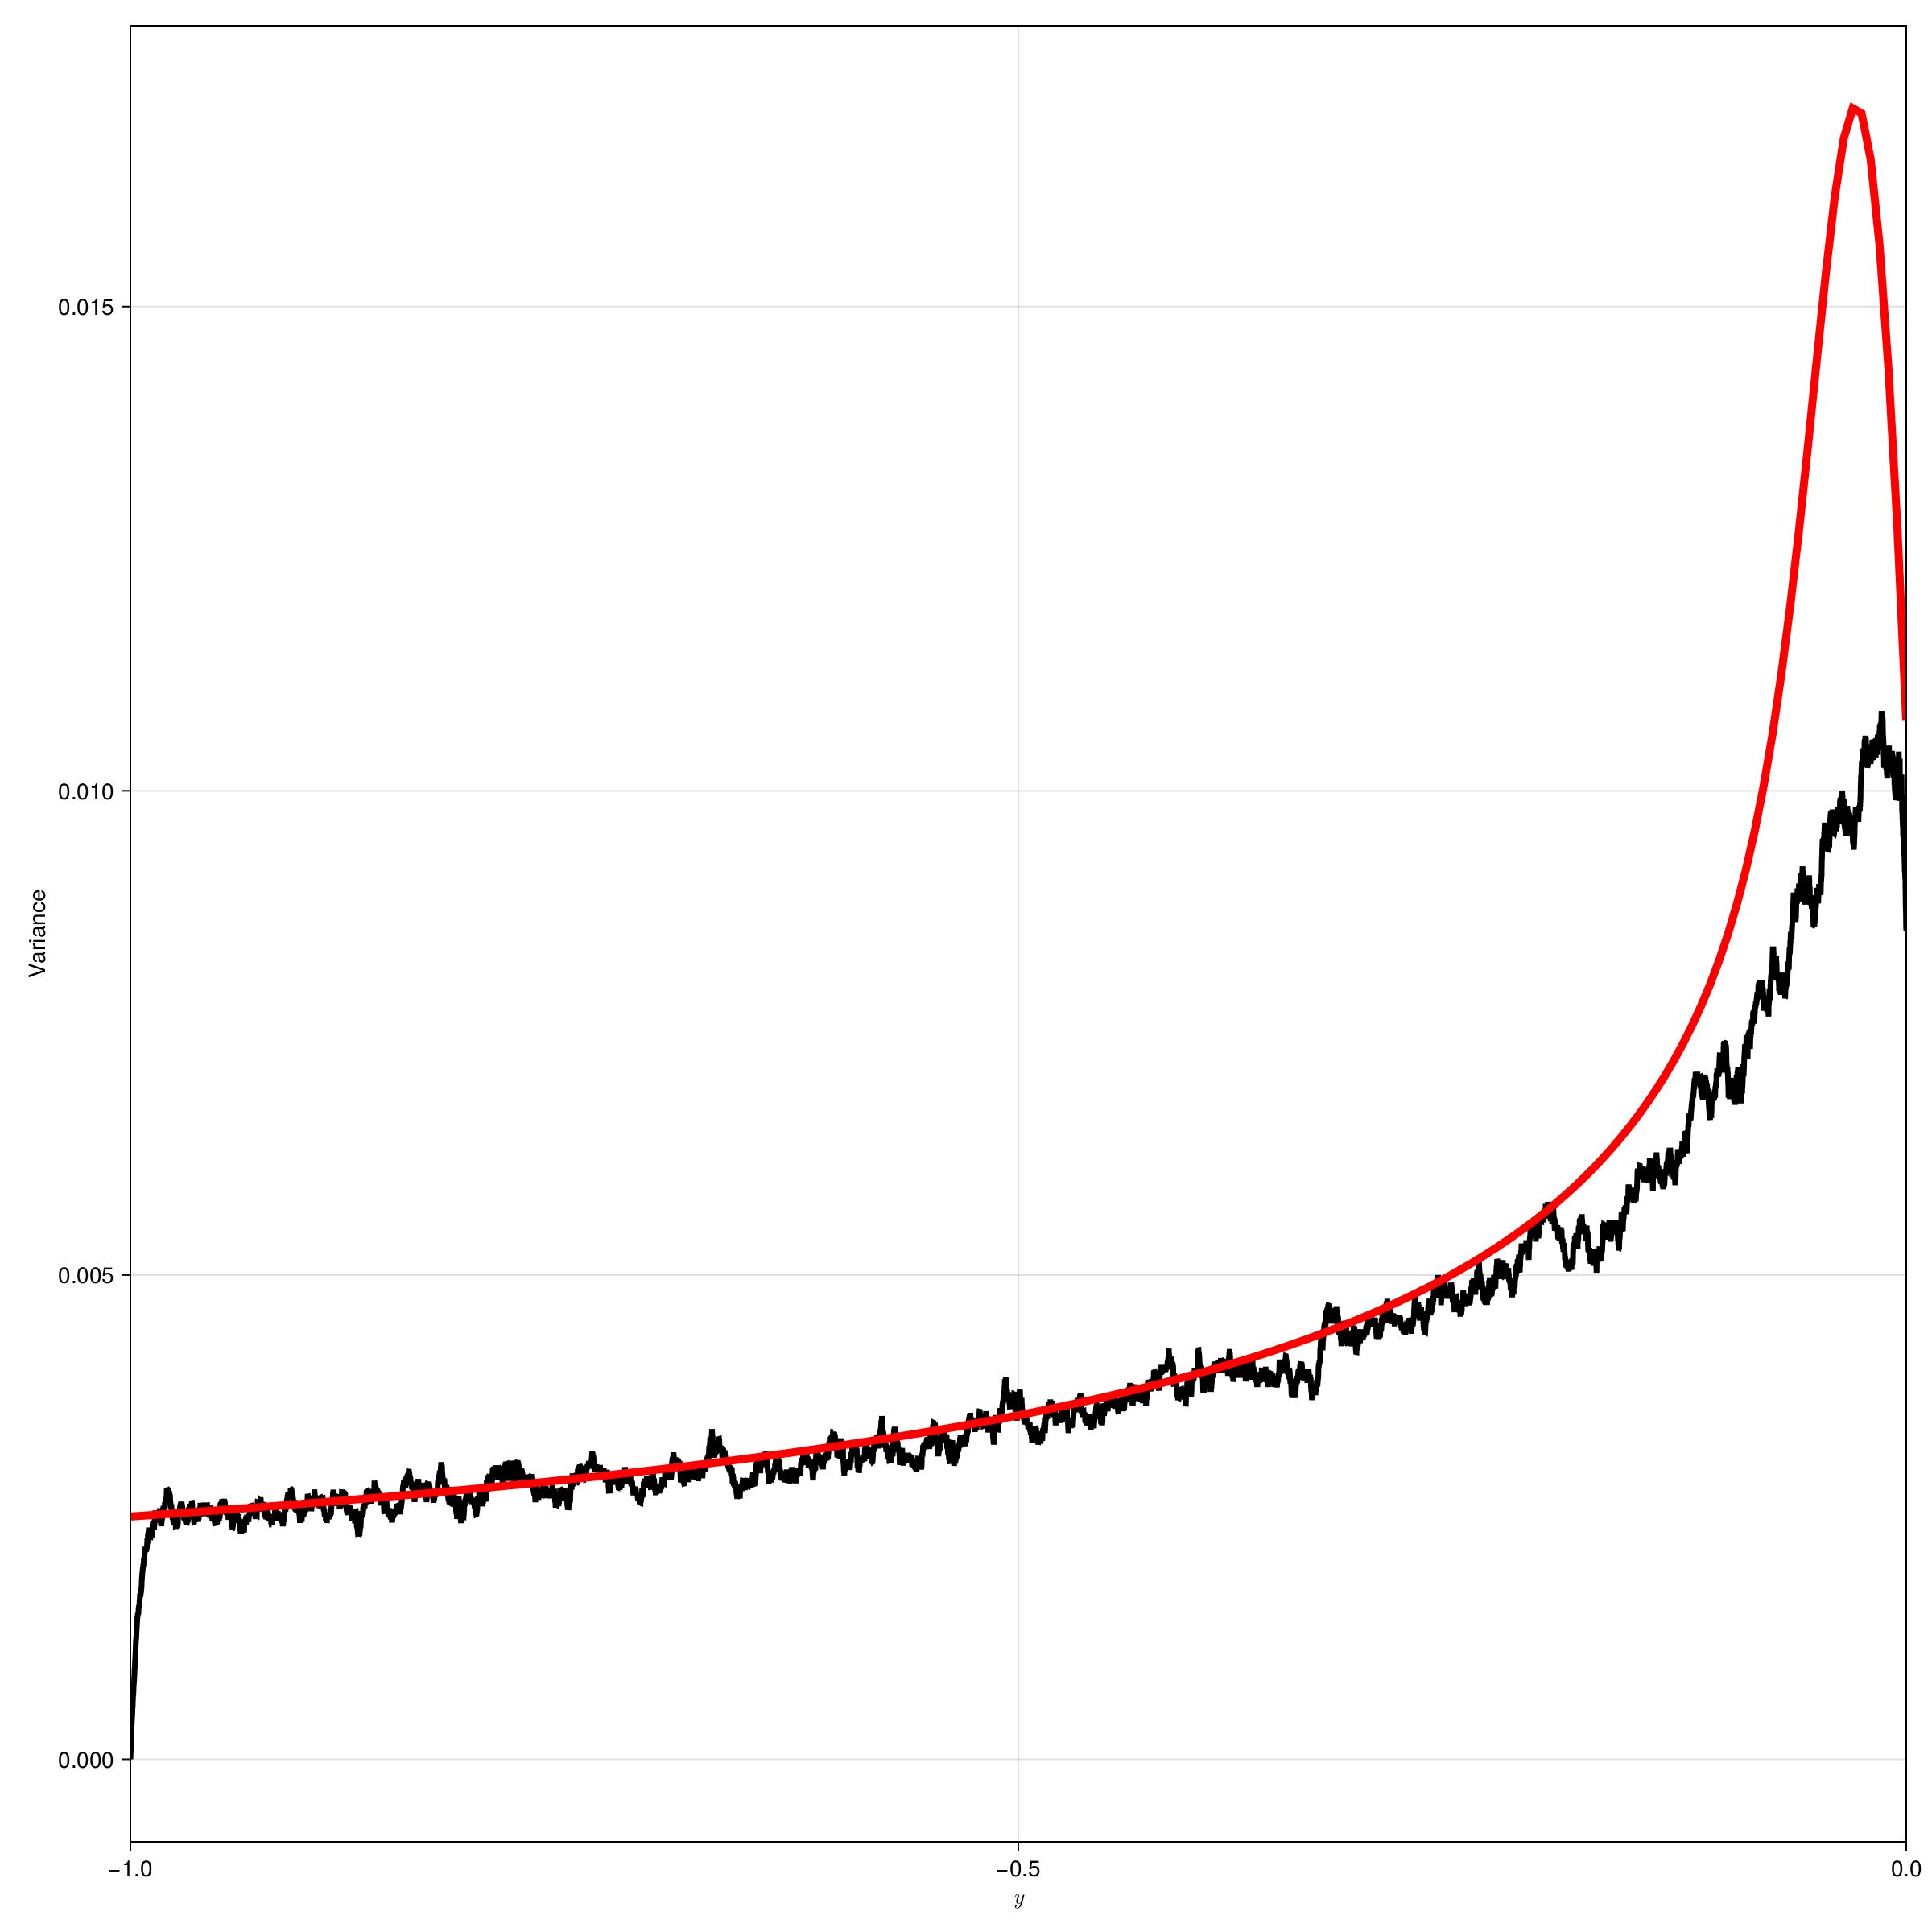
\includegraphics[keepaspectratio, width = \textwidth]{../figures/AddFoldVariance.png}
        \caption{}
        \label{fig1.8.a}
    \end{subfigure}
    \hfill 
    \begin{subfigure}[b]{0.3\textwidth}
        \centering 
        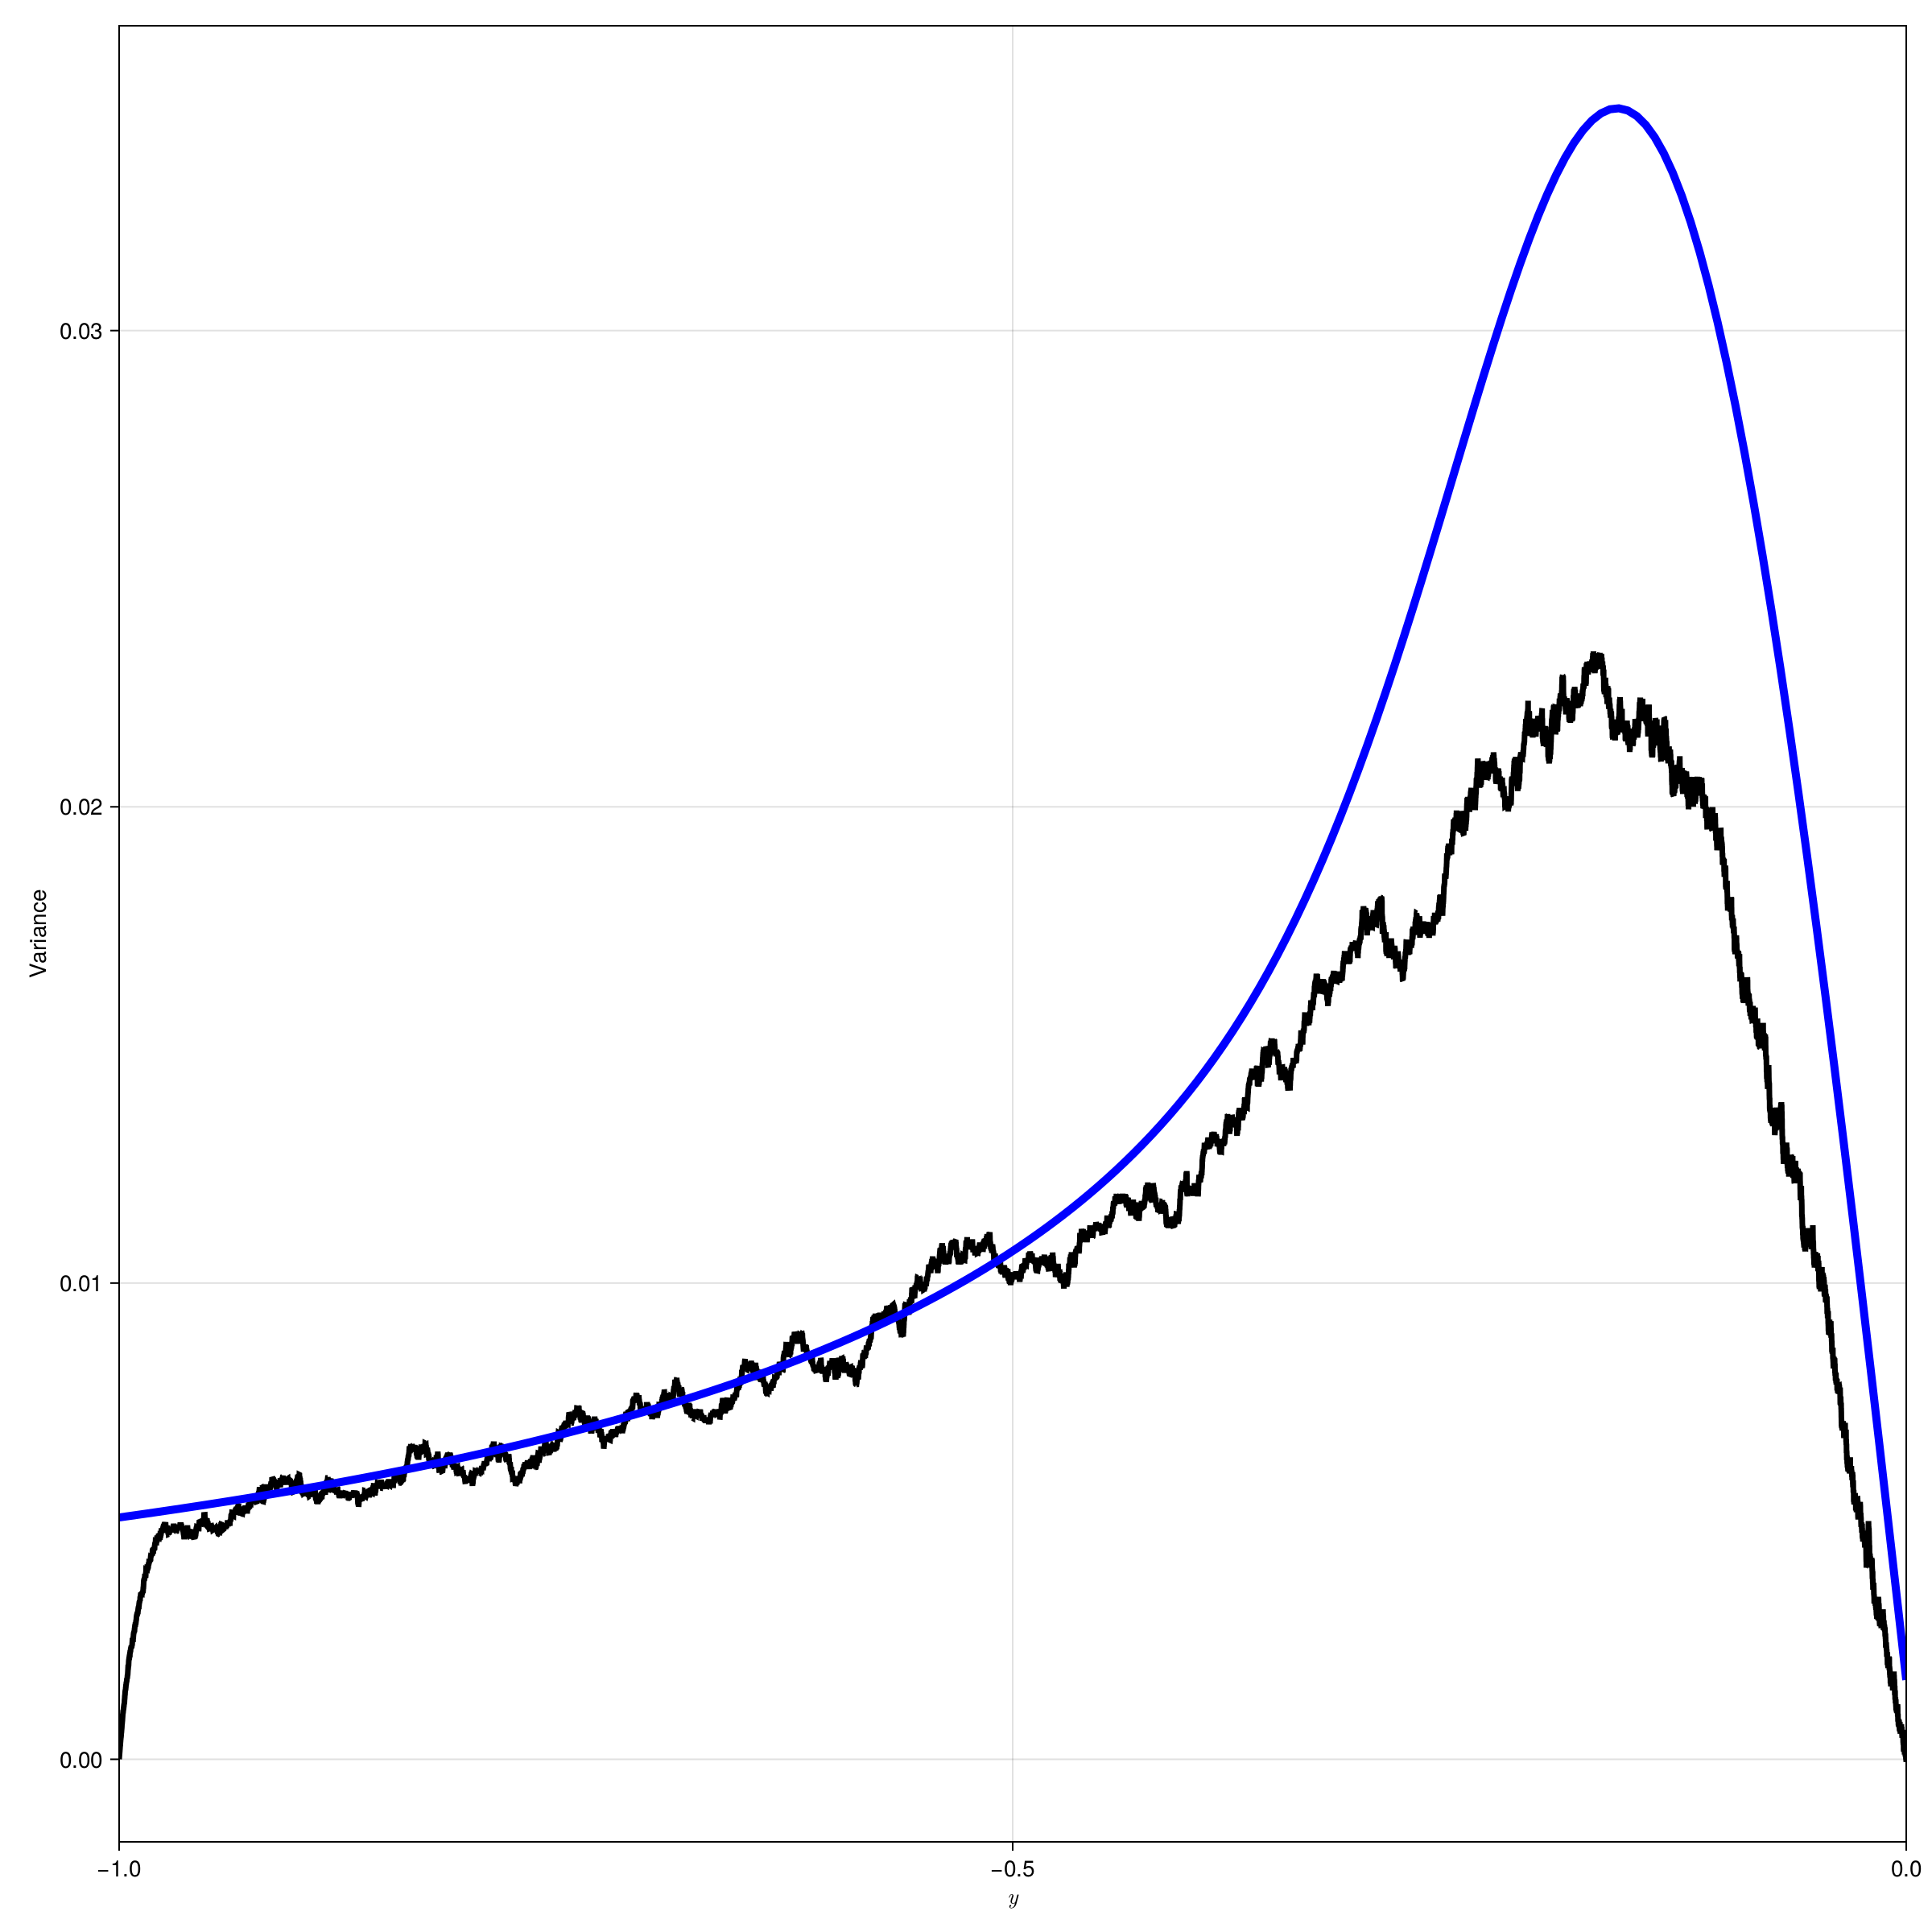
\includegraphics[keepaspectratio, width = \textwidth]{../figures/AddPitchVariance.png}
        \caption{}
        \label{fig1.8.b}
    \end{subfigure}
    \hfill
    \begin{subfigure}[b]{0.3\textwidth}
        \centering 
        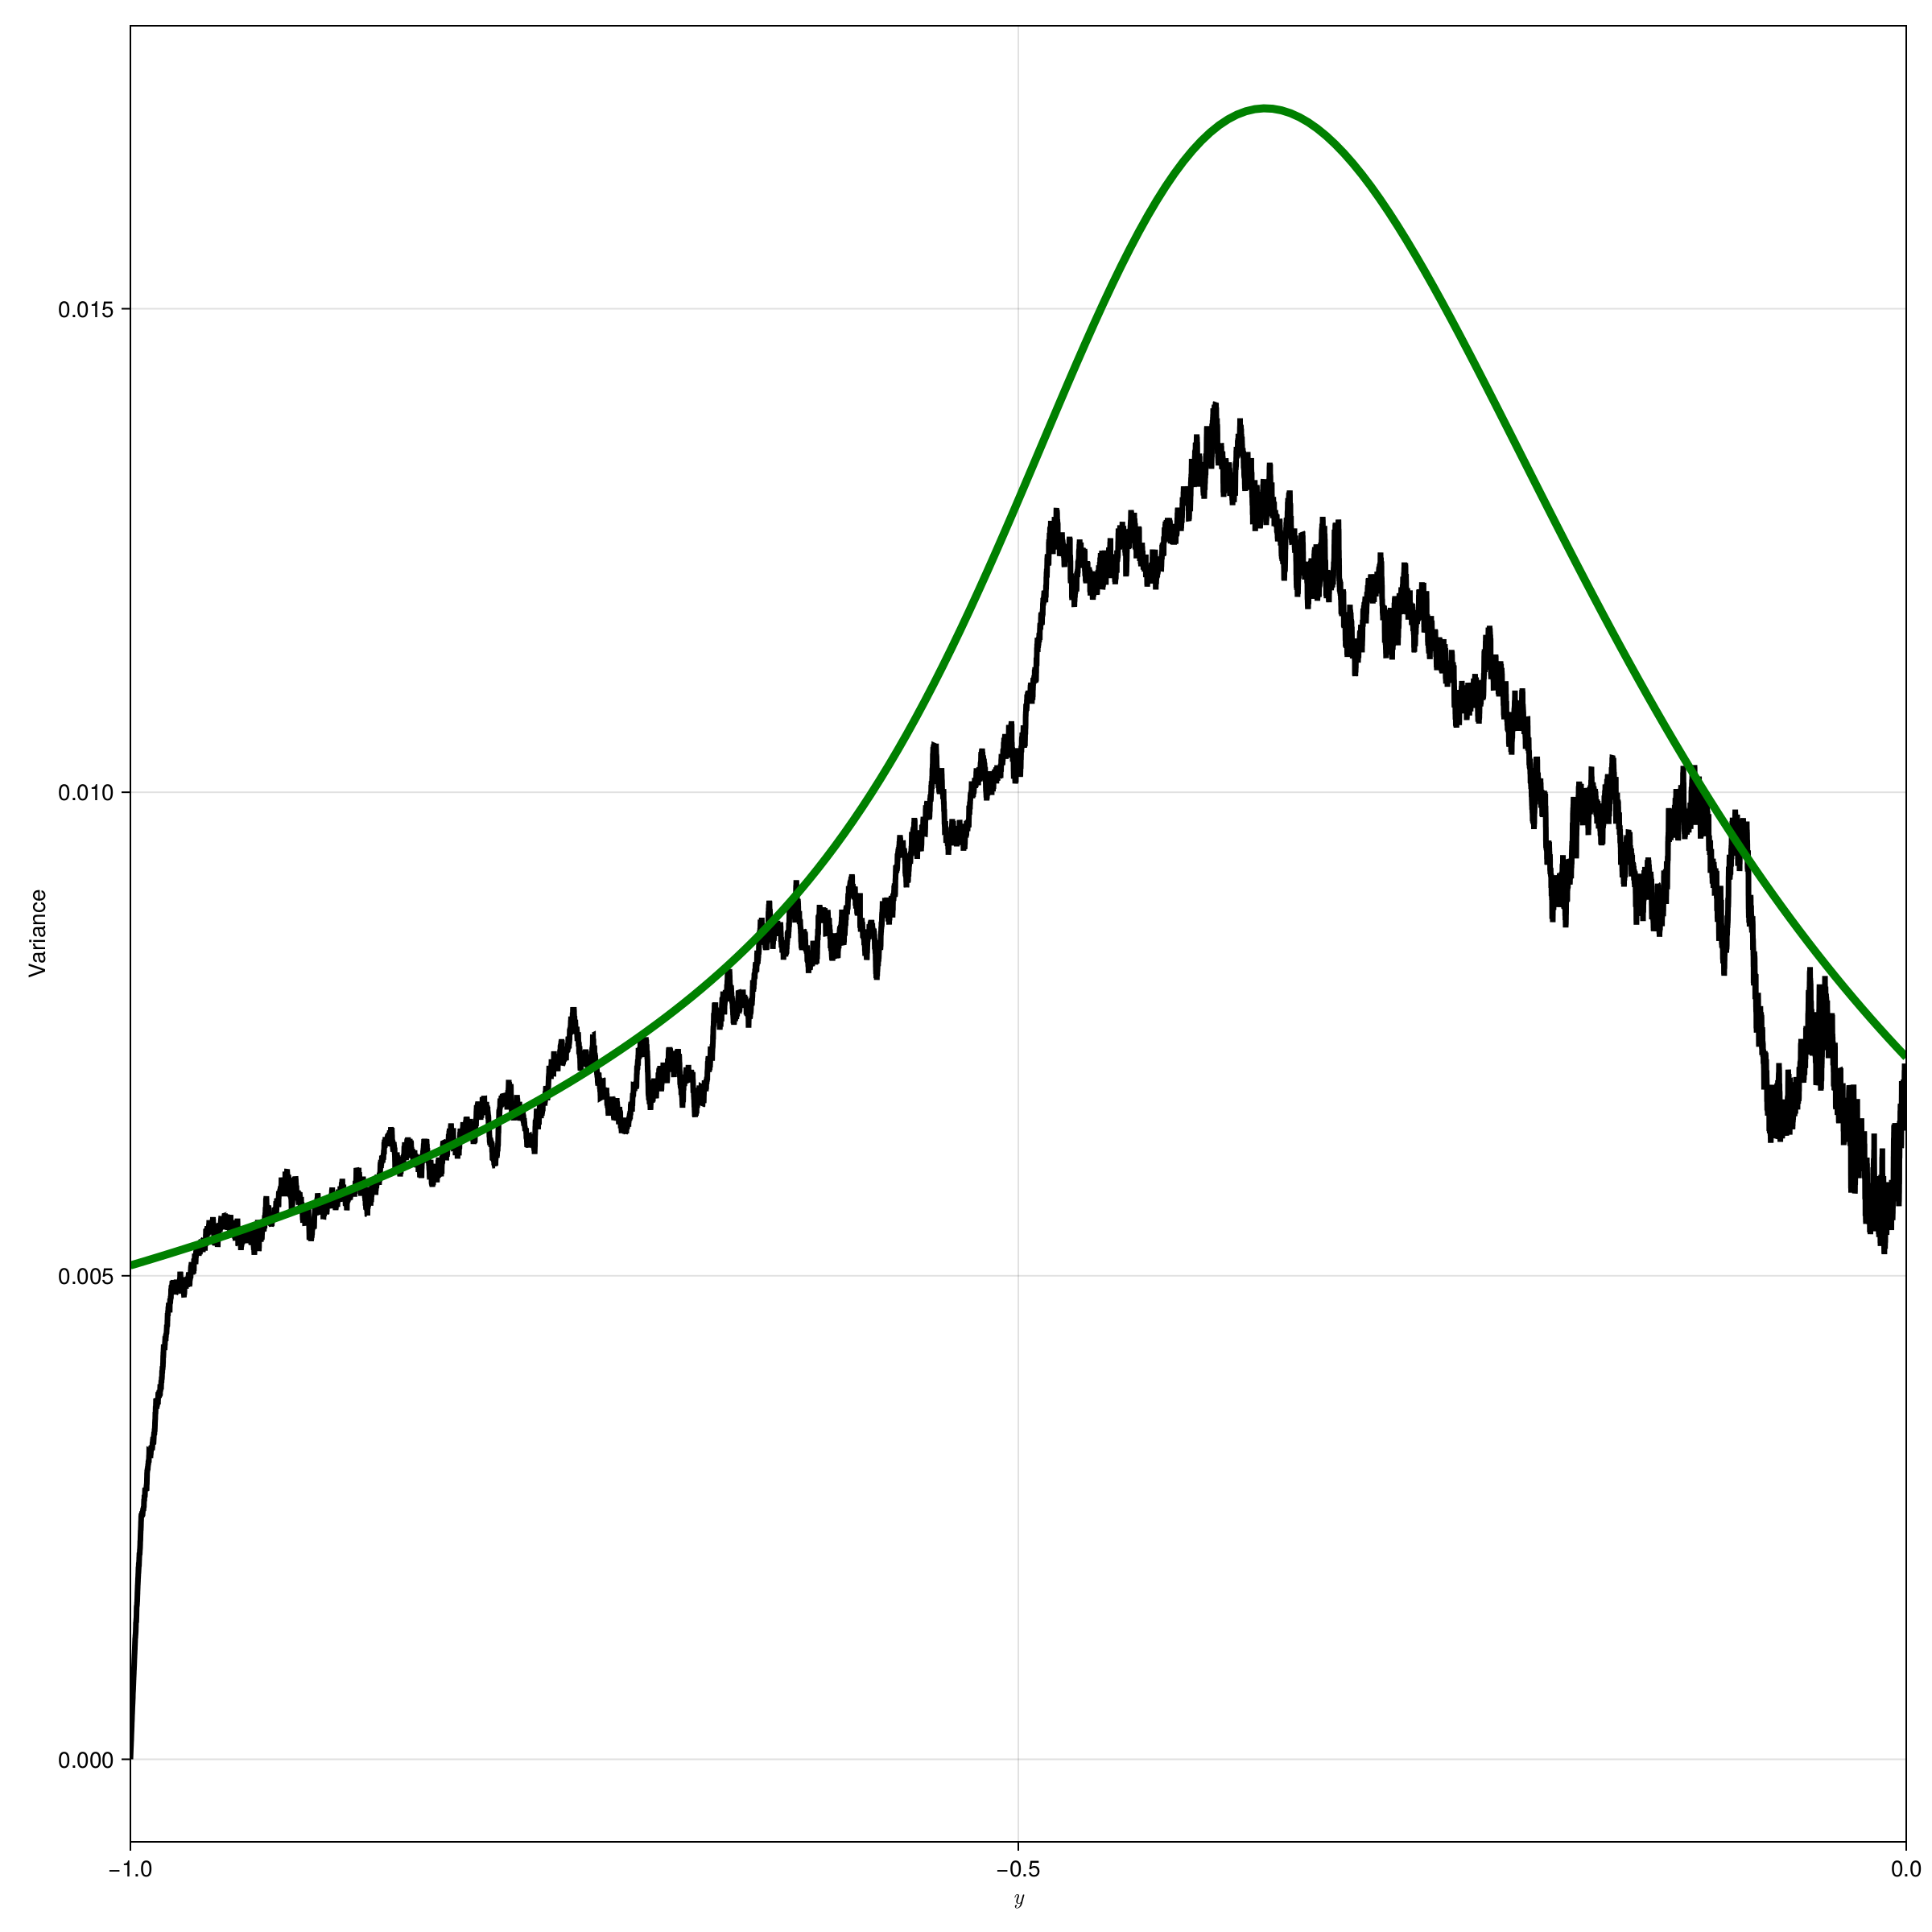
\includegraphics[keepaspectratio, width = \textwidth]{../figures/AddTransVariance.png}
        \caption{}
        \label{fig1.8.c}
    \end{subfigure}
    \caption{Comparison between the analytical variance of the stationary Fokker-Planck distribution of the fold (a), pitchfork (b) and transcritical (c) normal forms (colored lines) against the numerical variance of an ensemble of $1000$ sample paths (black lines) for the same cases (noise level $\sigma = 0.1$).}
    \label{fig1.8}
\end{figure}
One clear observation that we can gather from Figure \ref{fig1.8} is that in all three cases the (analytic) variance is non-monotonic and it reaches a local maxima in the proximity of the bifurcation at $y=0$ before decreasing. This apparent anomaly is a result of imposing reflecting boundary conditions for the probability current.
As a matter of fact for parameter values $y<<0$ away from the deterministic B-tipping, the effect of reflecting boundaries on the stationary distribution are negligible since, as we previously established, the stochastic process is topologically equivalent to the OUP and it stays bounded within the neighborhood of the slow critical manifold. 
As we approach the critical transition however the density $p_{s}(x; y)$ becomes more confined around the stable equilibria leading to N-tippings to occur with higher and higher probability. This can be easily verified by checking how decreasing the noise level $\sigma$ brings the local maxima of the variance closer and closer to the actual N-tipping at $y=0$.
The second most evident observation concerns the discrepancies between the analytical and numerical variance near the local maxima. In all three cases in fact we observe that the two curves agree when the parameter's values are far away from the deterministic critical transition however they largely differ as the parameter value gets closer to the local maxima for the analytical variance.
We can ascribe such discrepancy to the choice that we made earlier in counting ensemble sample paths as escaped the moment they cross the unstable equilibria. This corresponds to absorbing boundary conditions which quite substantially differ from the reflecting boundary conditions used in our stationary Fokker-Planck density especially when boundary and noise effects become dominant (i.e. close to the deterministic critical transition as the basin of attraction shrinks further and further in size).
This argument is validated further by observing how the discrepancy between analytical and numerical variance for the fold bifurcation is significantly less than those for the remaining two normal forms; based on this observation we expect fewer trajectories to escape the stable equilibria for the fold normal form and this is exactly what we observe in the ensemble simulations as depicted in Figure \ref{fig1.9}.
We finally note how, in reality, trajectories that cross the unstable equilibria can, in principle, still recover to the stable branch with low probability, which further corroborates our observations above.
\begin{figure}[H]
    \centering 
    \begin{subfigure}[b]{0.95\textwidth}
        \centering 
        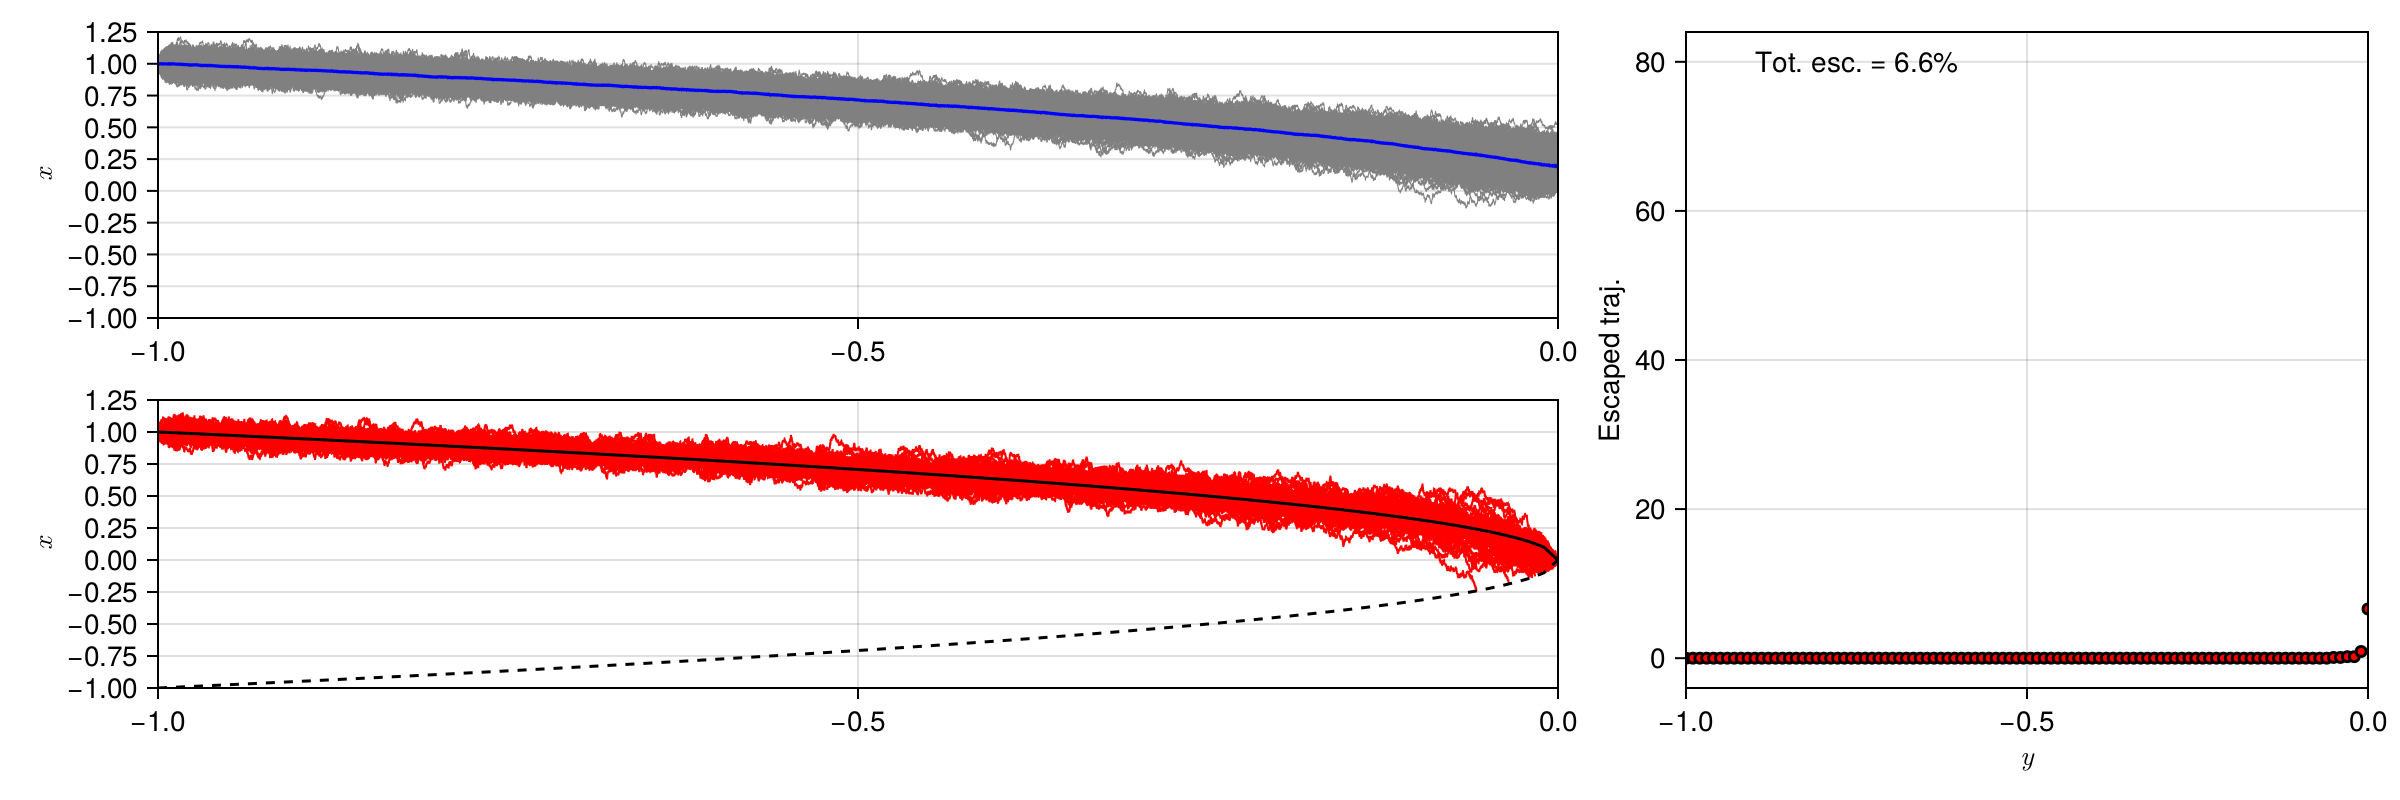
\includegraphics[keepaspectratio, width = \linewidth]{../figures/AddFoldEnsemble.png}
        \label{fig1.9.a}
    \end{subfigure}
    \hfill 
    \begin{subfigure}[b]{0.95\textwidth}
        \centering 
        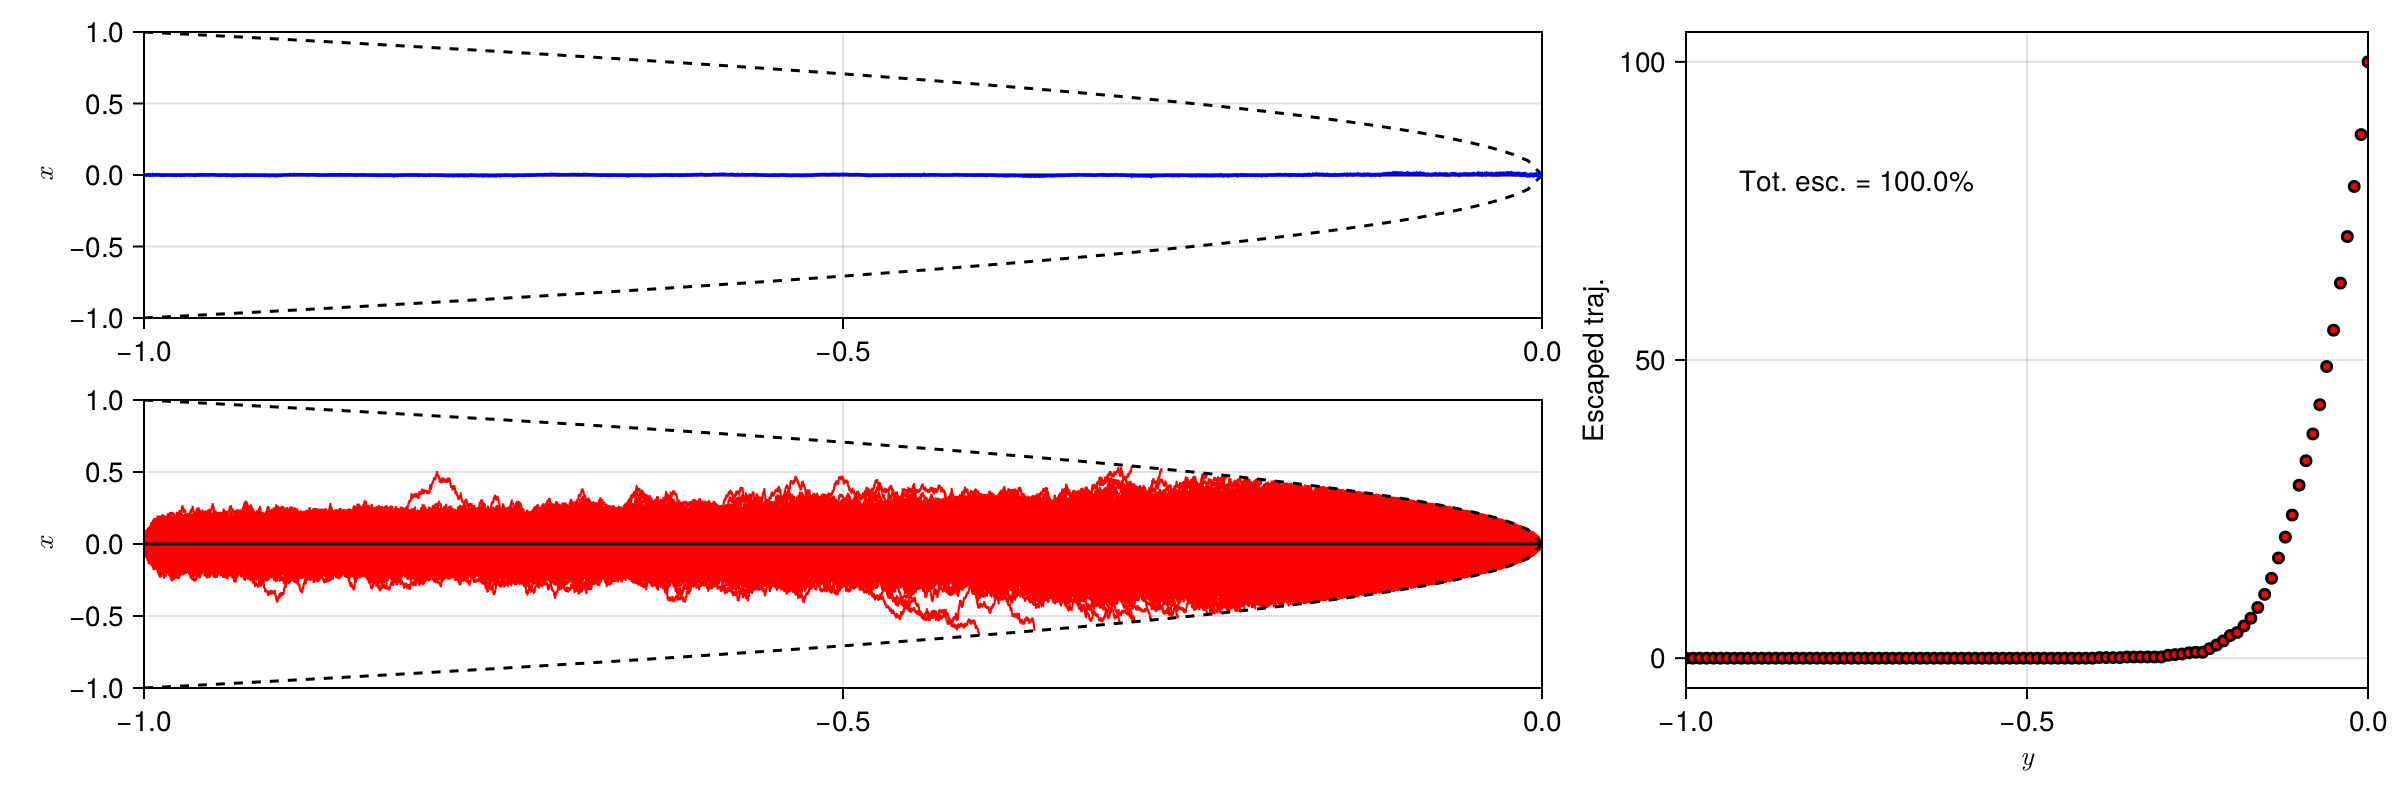
\includegraphics[keepaspectratio, width = \linewidth]{../figures/AddPitchEnsemble.png}
        \label{fig1.9.b}
    \end{subfigure}
    \hfill
    \begin{subfigure}[b]{0.95\textwidth}
        \centering 
        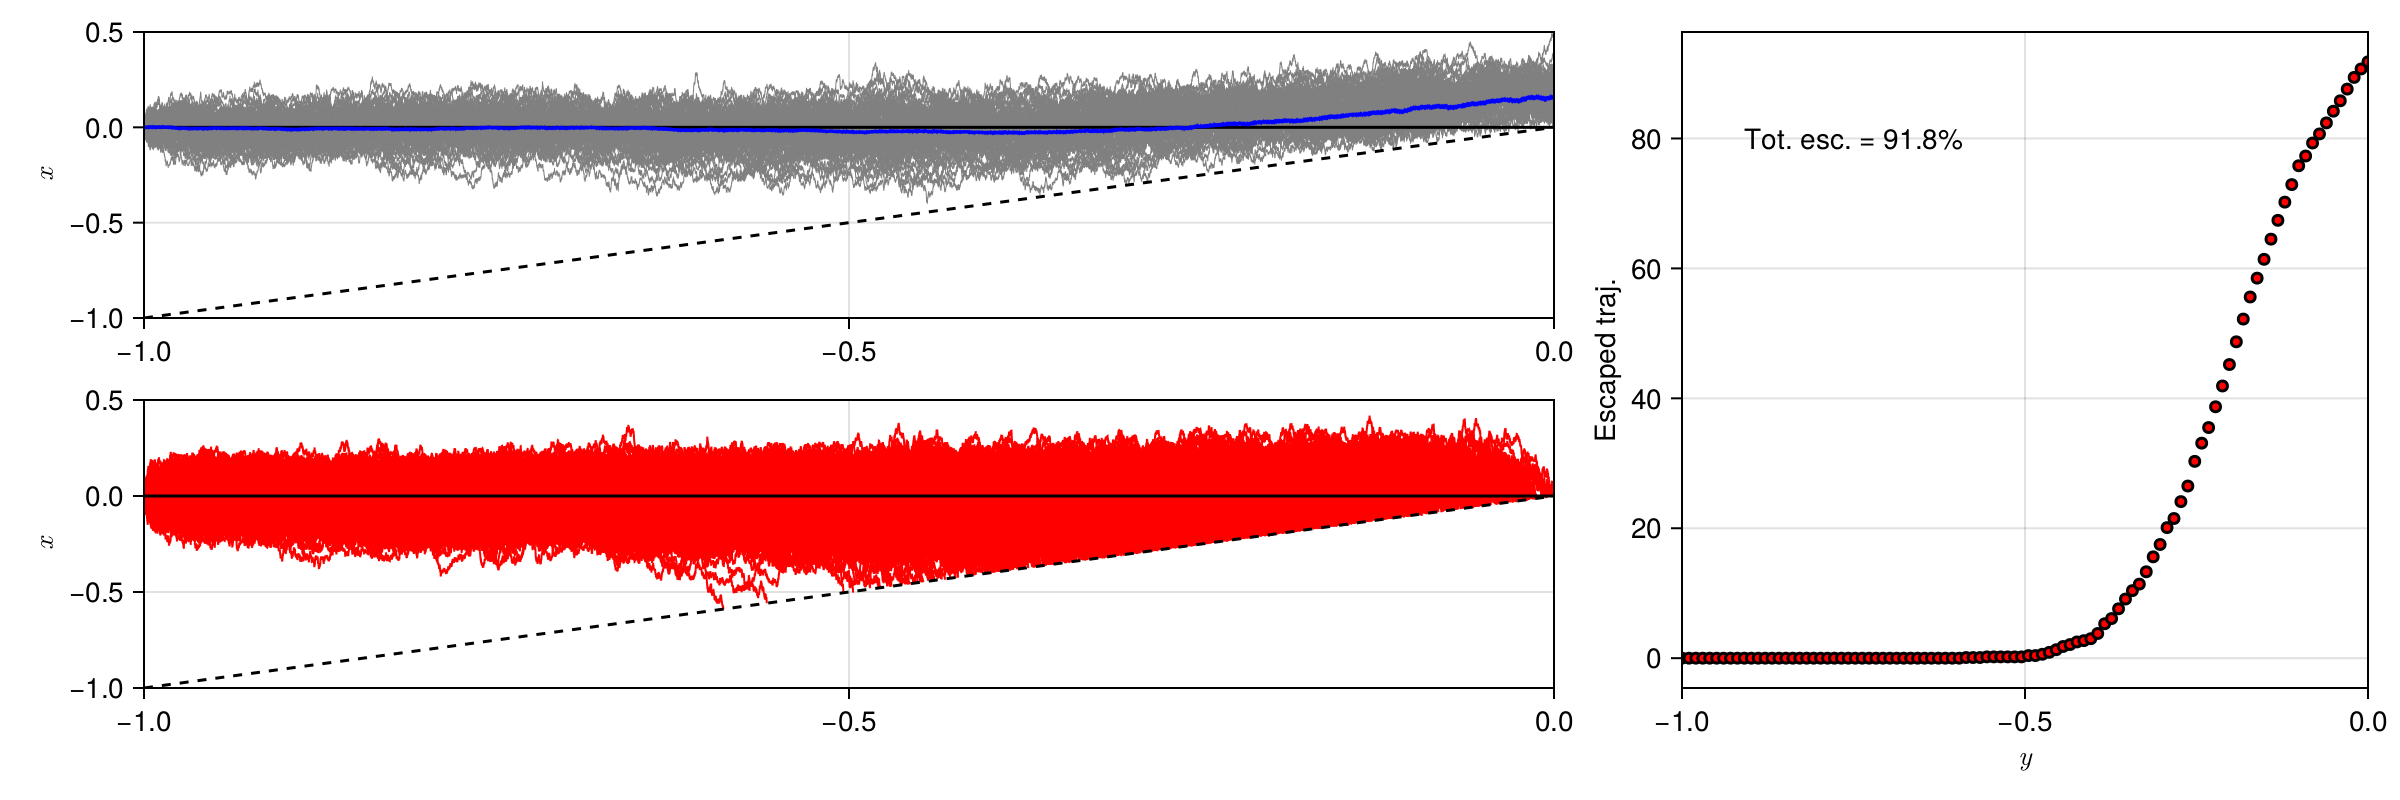
\includegraphics[keepaspectratio, width = \linewidth]{../figures/AddTransEnsemble.png}
        \label{fig1.9.c}
    \end{subfigure}
    \caption{Ensemble sample paths of fold (top), pitchfork (middle) and transcritical (bottom) normal forms showing separately the trajectories that stayed bounded on the stable branch of the critical manifold (gray lines, blue line shows the mean) prior to the bifurcation and those that escaped (red lines) beyond the unstable submanifold. On the left of each plot a percentage of the number of escaped trajectories at discrete values of $y$ is shown.}
    \label{fig1.9}
\end{figure}

\end{document}
